\documentclass{report}

\usepackage{geometry}
\geometry{a4paper,total={170mm,257mm},left=20mm,top=20mm}
\usepackage[utf8]{inputenc}
\usepackage{amsmath}
\usepackage{amsfonts}
\usepackage{amsthm}
\usepackage{amssymb}
\usepackage{bm}
\usepackage{graphicx}
\usepackage{paralist}
\usepackage[dvipsnames]{xcolor}
\usepackage{caption}
\usepackage{subcaption}
\usepackage{hyperref}
\hypersetup{urlbordercolor=ForestGreen,linkbordercolor=RoyalPurple}
\usepackage{tikz}
\usetikzlibrary{positioning}
\usetikzlibrary{intersections}
\usepackage{algpseudocode}
\usepackage{algorithm}
\usepackage{titling}
\usepackage{pgfplots}
\usepackage{fontawesome5}
 % Use the same header and libraries.
%%% Tento soubor obsahuje definice různých užitečných maker a prostředí %%%
%%% Další makra připisujte sem, ať nepřekáží v ostatních souborech.     %%%

%%% Drobné úpravy stylu

% Tato makra přesvědčují mírně ošklivým trikem LaTeX, aby hlavičky kapitol
% sázel příčetněji a nevynechával nad nimi spoustu místa. Směle ignorujte.
\makeatletter
\def\@makechapterhead#1{
  {\parindent \z@ \raggedright \normalfont
   \Huge\bfseries \thechapter. #1
   \par\nobreak
   \vskip 20\p@
}}
\def\@makeschapterhead#1{
  {\parindent \z@ \raggedright \normalfont
   \Huge\bfseries #1
   \par\nobreak
   \vskip 20\p@
}}
\makeatother

% Toto makro definuje kapitolu, která není očíslovaná, ale je uvedena v obsahu.
\def\chapwithtoc#1{
\chapter*{#1}
\addcontentsline{toc}{chapter}{#1}
}

% Trochu volnější nastavení dělení slov, než je default.
\lefthyphenmin=2
\righthyphenmin=2

% Zapne černé "slimáky" na koncích řádků, které přetekly, abychom si
% jich lépe všimli.
\overfullrule=1mm

%%% Makra pro definice, věty, tvrzení, příklady, ... (vyžaduje baliček amsthm)

\theoremstyle{plain}
\newtheorem{veta}{Věta}
\newtheorem{lemma}[veta]{Lemma}
\newtheorem{tvrz}[veta]{Tvrzení}

\theoremstyle{plain}
\newtheorem{definice}{Definice}
\newtheorem*{pozor}{Pozorování}
\newtheorem*{cvic}{Cvičení}
\newtheorem*{fakt}{Fakt}

\theoremstyle{remark}
\newtheorem*{dusl}{Důsledek}
\newtheorem*{pozn}{Poznámka}
\newtheorem*{prikl}{Příklad}

\theoremstyle{plain}
\newtheorem{thm}{Theorem}
%\newtheorem{lemma}[thm]{Lemma}
\newtheorem{claim}[thm]{Claim}

\theoremstyle{plain}
\newtheorem{defn}{Definition}
\newtheorem*{observ}{Observation}
\newtheorem*{exerc}{Exercise}
\newtheorem*{fact}{Fact}

\theoremstyle{remark}
\newtheorem*{cor}{Corollary}
\newtheorem*{rem}{Remark}
\newtheorem*{example}{Example}


%%% Prostředí pro důkazy

\newenvironment{dukaz}{
  \par\medskip\noindent
  \textit{Důkaz}.
}{
\newline
\rightline{$\qedsymbol$}
}

\newenvironment{myproof}{
	\par\medskip\noindent
	\textit{Proof}.
}{
	\newline
	\rightline{$\qedsymbol$}
}


%%% Prostředí pro sazbu kódu, případně vstupu/výstupu počítačových
%%% programů. (Vyžaduje balíček fancyvrb -- fancy verbatim.)

\DefineVerbatimEnvironment{code}{Verbatim}{fontsize=\small, frame=single}

%%% Prostor reálných, resp. přirozených čísel
\newcommand{\R}{\mathbb{R}}
\newcommand{\N}{\mathbb{N}}
\newcommand{\Z}{\mathbb{Z}}

%%% Užitečné operátory pro statistiku a pravděpodobnost
\DeclareMathOperator{\pr}{\textsf{P}}
\DeclareMathOperator{\E}{\textsf{E}\,}
\DeclareMathOperator{\var}{\textrm{var}}
\DeclareMathOperator{\sd}{\textrm{sd}}

%%% Příkaz pro transpozici vektoru/matice
\newcommand{\T}[1]{#1^\top}

%%% Vychytávky pro matematiku
\newcommand{\goto}{\rightarrow}
\newcommand{\gotop}{\stackrel{P}{\longrightarrow}}
\newcommand{\maon}[1]{o(n^{#1})}
\newcommand{\abs}[1]{\left|{#1}\right|}
\newcommand{\dint}{\int_0^\tau\!\!\int_0^\tau}
\newcommand{\isqr}[1]{\frac{1}{\sqrt{#1}}}

%%% Vychytávky pro tabulky
\newcommand{\pulrad}[1]{\raisebox{1.5ex}[0pt]{#1}}
\newcommand{\mc}[1]{\multicolumn{1}{c}{#1}}


% set up \maketitle to accept a new item
\predate{\begin{center}\placetitlepicture\large}
	\postdate{\par\end{center}}

% commands for including the picture
\newcommand{\titlepicture}[2][]{%
	\renewcommand\placetitlepicture{%
		\includegraphics[#1]{#2}\par\medskip
	}%
}
\newcommand{\placetitlepicture}{} % initialization

 % Use global macros.

\usepackage{babel}

\title{Geometrická reprezentace grafů}
\author{Tomáš Turek}
\titlepicture[width=6in]{res/filament}
\date{\today}

\begin{document}
	\maketitle
	
	\INFO{Many parts of text are taken from the handouts made by Jan Kratochvíl. I also add some of my notes from the lectures and some pictures.}
	
	\tableofcontents
	\part{Geometrická reprezentace grafů I}
	\chapter{Introduction}

Firstly we remind some basics from flows and cuts. 

\section{Network flow}

\textbf{Flow} is defined on a \textbf{network}. Network is on a oriented graph $G = (V,E)$ and it has two special vertices $s,t \in V$ called source and target. Also we have a capacity, which is a mapping $c : E \to \R_{0}^{+}$. Flow then is a mapping $f : E \to \R_{0}^{+}$ which has two properties.

\begin{enumerate}
	\item $\forall e \in E: f(e) \leq c(e)$
	\item Kirchoff's law: $\forall v \neq s, t \in V: \sum_{uv \in E} f(uv) - \sum_{vu \in E} f(vu) = 0$
\end{enumerate}

\section{Min $s,t$-cut}

Now we also remind ourselves another term which is an $s,t$-cut. Which is a $M \subset E$ such that no $s,t$-path exists in $G' = (V, E \setminus M)$.

These basic terms can be generalized to a \textbf{multi-commodity flow} problem and \textbf{multi-cut} problem.
	\chapter{Interval, permutation and function graphs}

\section{Interval graphs}

\begin{defn}
	A graph is an \textbf{interval graph} if it is isomorphic to the intersection graph of a collection of intervals on a line.
\end{defn}

\begin{observ}
	Every interval graph has an interval representation in which all of the intervals are closed.
\end{observ}

\begin{defn}[Clique-path decomposition]
	A \textbf{clique-path decomposition} of a graph is a clique-tree decomposition in which the underlying tree is a path.
\end{defn}

\begin{thm}
	For any graph $G$, the following statements are equivalent:
	
	\begin{enumerate}
		\item $G$ is an interval graph,
		\item $G$ has a clique-path decomposition, and
		\item $G$ is an intersection graph of subpaths of a path.
	\end{enumerate}
\end{thm}

\begin{proof}
	"$1. \Leftrightarrow 3.$" is obvious.
	
	"$1. \Rightarrow 2.$" Assume $I_u , u \in V(G$ is an interval representation of $G$. Use the fact that intervals on a line have the Helly property, i.e., if any two of a collection of intervals have a nonempty intersection, then all of them have a nonempty intersection. In other words, if $Q_i \in \mathcal{Q}$ is a maximal clique of $G$, then there exists a point $P_i$ which belongs to $\bigcap_{u \in Q_i} I_u$ . Moreover, for every $v \notin Q_i , P_i \notin I_v$, since $Q_i$ is a maximal clique. (E.g., the rightmost of the left endpoints of the intervals $I_u , u \in Q_i$ is a good candidate for $P_i$.) Order the cliques of $Q$ as $Q_1, Q_2, \dots, Q_k$ so that $P_1 < P_2 < \dots < P_k$. Then the path
	$Q_1 Q_2 \dots Q_k$ is a clique-path decomposition of $G$.
	
	"$2. \Rightarrow 3.$" Given a clique-path decomposition $P = (\mathcal{Q}, F)$, define $P_u = P [\{Q : u \in Q \in \mathcal{Q}\}]$ for $u \in V(G)$. Clearly $V(P_u) \cap V(P_v) \neq \emptyset$ iff $u$ and $v$ belong to the same maximal clique of $G$, which happens if and only $u$ and $v$ are adjacent in $G$.
\end{proof}

\section{Comparability graphs}

\begin{defn}
	A graph $G$ is a \textbf{comparability graph} if there exists a partial order $P = (V(G), \leq)$ on the vertex set of $G$ (i.e., an \textbf{antireflexive}, \textbf{antisymmetric} and \textbf{transitive binary relation}) such that for any two vertices $u, v \in V(G)$, $uv \in E(G)$ if and only if $u \leq v$ or $v \leq u$ (i.e., if $u$ and $v$ are comparable in $P$). The class of comparability graphs will be denoted by CO.
\end{defn}

\begin{observ}
	A graph is a comparability graph if and only if its edges can be transitively oriented.
\end{observ}

\begin{notation}
	If $\mathcal{A}$ is a graph class, the symbol $\text{co}-\mathcal{A}$ is used to denote the class containing the complements of the graphs in $\mathcal{A}$.
\end{notation}

\begin{observ}
	If $A \subseteq B$, then $\text{co}-A \subseteq \text{co}-B$.
\end{observ}

\begin{thm}
	All equivalencies hold:
	
	\begin{enumerate}
		\item $\text{FUN} = \text{co}-\text{CO}$
		\item $\text{PER} = \text{CO} \cap \text{co}-\text{CO}$
		\item $\text{INT} = \text{CHOR} \cap \text{co}-\text{CO}$
	\end{enumerate}
\end{thm}

\begin{proof}
	\begin{enumerate}
		\item ”FUN $\subseteq$ co-CO”: Given a collection of curves joining two vertical parallel lines (and lying in the stripe between them), for any two non-crossing curves, it is uniquely determined which one lies above the other one (this follows from the Jordan curve theorem), and this gives a transitive orientation of the complement of the intersection graph of this collection.
		
		”co-CO $\subseteq$ FUN”: Let $G = (V, E)$ be a graph and let $P = (V, \leq)$ be a partial order which corresponds to a transitive orientation of the complement of $G$. If $d$ is the dimension of $P$, $P$ is the intersection of $d$ linear orders $L_1, L_2 , \dots, L_d$ of $V$. In the plane, draw d distinct parallel (vertical) lines $l_1, l_2, \dots, l_d$, and on each $l_i$ , mark distinct points $P_{iu}, u \in V$ bottom up in the order $L_i$. Consider piece-wise linear curves $c(u) = P_{1u} P_{2u} \dots P_{du}$, for $u \in V$. If $uv \in E$, $u$ and $v$ are incomparable in $P$,	and hence there are indices $i$ and $j$ such that $u <_{L_i} v$ and $v <_{L_j} u$, in other words $P_{iu}$ is below $P_{iv}$, while $P_{ju}$ is above $P_{jv}$. Hence the curves $c(u)$ and $c(v)$ cross somewhere between $l_i$ and $l_j$. If, on the other hand, $uv \notin E$, $uv$ is an edge of the complement of $G$ and hence $u$ and $v$ are comparable in $P$, say, $u \leq v$. But then $u <_{L_i} v$ for every $i = 1, 2, \dots, d$, and for each $i = 1, 2, \dots, d - 1$, the curve $c(u)$	lies below the curve $c(v)$ in the stripe between $l_i$ and $l_{i+1}$. Thus $c(u)$ and $c(v)$ are disjoint.
		
		\item Note first that co-PER $\subseteq$ PER. Indeed, given a permutation representation of a graph, swap	the order of the endpoints on one of the bounding lines to obtain a representation of the complement of the given graph. Then PER $=$ co-(co-PER) $\subseteq$ co-PER, and hence PER $=$ co-PER.
		
		”PER $\subseteq$ CO $\cap$ co-CO”: Obviously PER $\subseteq$ FUN $=$ co-CO. Then the above small observation implies PER $=$ co-PER $\subseteq$ co-(co-CO) $=$ CO as well.

		”CO $\cap$ co-CO $\subseteq$ PER”: Suppose both $G$ and its complement can be transitively oriented, say $\overrightarrow{E_1}$ be a transitive orientation of $G$ and $\overrightarrow{E_2}$ a transitive orientation of the complement $-G$ of $G$. Then $\overrightarrow{E_1} \cup \overrightarrow{E_2}$ is a transitive orientation of the complete graph $K_{V(G)}$ on the vertex set of $G$, i.e., a linear ordering of the vertices of $G$. And so is $\overrightarrow{E_1}^{-1} \cup \overrightarrow{E_2}$. Place the vertices of $G$ on two parallel lines, on one of them in the linear order given by $\overrightarrow{E_1} \cup \overrightarrow{E_2}$, on the other one in the order given by $\overrightarrow{E_1}^{-1} \cup \overrightarrow{E_2}$, and connect the two occurrences of a vertex $u$ by a straight-line segment called $s(u)$, for every vertex $u \in V(G)$. If $uv \in E(G)$, then the pair $u, v$ is ordered differently on the two lines (by $\overrightarrow{E_1}$ on one of them and by $\overrightarrow{E_1}^{-1}$ on the other one) and the segments $s(u), s(v)$ cross each other somewhere between	the two lines. If $uv \notin E(G)$, the pair $u, v$ is ordered the same way (by $\overrightarrow{E_2}$) on both of the lines, and thus the segments $s(u)$ and $s(v)$ are disjoint. So $\{s(u)\}_{u \in V(G)}$ is a permutation representation of $G$.
		
		\item ”INT $\subseteq$ CHOR $'cap$ co-CO”: Let $\{I(u)\}_{u \in V(G)}$ be an interval representation of a graph $G$. Define a transitive orientation $\overrightarrow{E_2}$ of the non-edges of $G$ by setting $uv \in \overrightarrow{E_2}$ if $\max I(u) < \min I(v)$. Thus $G \in$ co-CO. The fact that $G \in$ CHOR follows from the fact that
		
		$$
		\text{INT} = \mathcal{IG}(\{\text{connected subgraphs of paths}\}) \subseteq
		$$
		
		$$
		\subseteq \mathcal{IG}(\{\text{connected subgraphs of trees}\}) = \text{CHOR}.
		$$
		
		”CHOR $\cap$ co-CO $\subseteq$ INT”: Let $G$ be a chordal graph which allows a transitive orientation $\overrightarrow{E_2}$ of its non-edges. Define a binary relation $<$ on the set $\mathcal{Q}$ of maximal cliques of $G$ by setting
		
		$$
		Q < Q' \Leftrightarrow \exists u \in Q \exists v \in Q' : uv \in \overrightarrow{E_2}.
		$$
		
		\begin{claim}
			The relation $<$ is a partial order on $\mathcal{Q}$.
		\end{claim}
		
		\begin{proof}[Proof of claim]
			We will show all properties of partial order.
			\begin{itemize}
				\item Antireflexivity: Each $Q \in \mathcal{Q}$ is a clique, so there are no two vertices $u, v \in Q$ that would form a	non-edge of $G$. Hence $Q \not< Q$.
				
				\item Antisymmetry: Suppose for the contrary that there are $u \in Q, v \in Q'$ s.t. $uv \in \overrightarrow{E_2}$, and another pair $x \in Q, y \in Q'$ s.t. $yx \in \overrightarrow{E_2}$. First observe that $u \neq x$ and $v \neq y$ (if $u = x$, the transitivity of $\overrightarrow{E_2}$ would imply $yv \in \overrightarrow{E_2}$, which is impossible; if $v = y$, the transitivity of $\overrightarrow{E_2}$ would imply $ux \in \overrightarrow{E_2}$, which is again impossible). Next observe that both $uy$ and $xv$ must be edges of $G$ (if $uy \notin E(G)$, then either $uy \in \overrightarrow{E_2}$, or $yu \in \overrightarrow{E_2}$, yielding $ux \in \overrightarrow{E_2}$ in the former case and $yv \in \overrightarrow{E_2}$ in the letter one, both contradicting the fact that $Q$ and $Q'$ are cliques of $G$; the case of $xv \notin E(G)$ is analogous). Lastly, we conclude that $G[\{u, v, x, y\}] \simeq C_4$ , contradicting the assumption that $G$ is chordal.
				
				\item Transitivity: Suppose $Q < Q' < Q''$ and let $u \in Q, v, x \in Q'$ and $y \in Q''$ be vertices such that $uv, xy \in \overrightarrow{E_2}$. If $v = x$, the transitivity of $\overrightarrow{E_2}$ implies $uy \in \overrightarrow{E_2}$, hence $Q < Q''$. If $v \neq x$, one of $ux$, $vy$
				must be a non-edge (otherwise $G[\{u, v, x, y\}]$ would be an induced cycle of length 4, contradicting the assumption that $G$ is chordal). If $ux \notin E(G)$, $ux \in \overrightarrow{E_2}$ and the transitivity of $\overrightarrow{E_2}$ implies $uy \in \overrightarrow{E_2}$. If $vy \notin E(G)$, $vy \in \overrightarrow{E_2}$ and the transitivity of $\overrightarrow{E_2}$ implies $uy \in \overrightarrow{E_2}$. In either case, $Q < Q''$.
			\end{itemize}
		\end{proof}
		
		\begin{claim}
			The relation $<$ is a linear ordering of $\mathcal{Q}$.
		\end{claim}
		
		\begin{proof}[Proof of claim]
			Let $Q \neq Q'$ be two different maximal cliques of $G$. Their maximality implies that none of them is a subset of the other one. Hence there is a vertex $u \in Q$ which does not belong to $Q'$ . If $u$ were adjacent to all vertices of $Q'$, $Q' \cup \{u\}$ would be a clique of $G$, contradicting the maximality of $Q'$ . Hence there is a $v \in Q'$ such that $uv \notin E(G)$. Then either $uv \in \overrightarrow{E_2}$ or $vu \overrightarrow{E_2}$, thus $Q < Q'$ or $Q' < Q$.
		\end{proof}
		
		\begin{claim}
			Let $\mathcal{Q} = \{Q_1 < Q_2 < \dots < Q_k\}$ be the maximal cliques of $G$ ordered by $<$. Then $P_G = (\mathcal{Q}, \{Q_i Q_{i+1}: i = 1, 2, \dots, k - 1\})$ is a clique-path decomposition of $G$, and hence $G \in$ INT.
		\end{claim}
		
		\begin{proof}[Proof of claim]
			Indeed $P_G$ is a path whose nodes are the maximal cliques of $G$. It remains to show that vertices of $G$ appear in these cliques consecutively. Suppose $Q < Q' < Q''$ and $u \in Q \cap Q''$. If there were a vertex $v \in Q'$ nonadjacent to $u$, we would have $uv \in \overrightarrow{E_2}$ because of $Q < Q'$ and $vu \in \overrightarrow{E_2}$ because of $Q' < Q''$, contradicting the antisymmetry of $\overrightarrow{E_2}$. Hence $u$ is adjacent to all vertices of $Q'$ , and thus
			$u \in Q'$ follows from the maximality of $Q'$.
		\end{proof}
	\end{enumerate}
\end{proof}
	\chapter{Interval filament graphs}

\begin{defn}
	Given a half-plane $\pi$ with a border-line $l$, an \textbf{interval filament} in $\pi$ is a simple curve with
	endpoints on $l$, its interior lying in $\pi$ and within the stripe determined by lines perpendicular to $l$ and
	passing through the endpoints of the curve. The class of \textbf{interval filament graphs} is $\text{IFA} = \mathcal{IG}\{\text{interval filaments in a half-plane}\}$.
\end{defn}

\begin{figure}[!ht]\centering
	\begin{tikzpicture}
		\draw[color = gray] (2,0) -- (10,0);
		\node at (3,.3) {$l$};
		\draw[color=black, thick] (5,.01) edge (10,.01);
		\draw[dotted] (5,0) edge (5, 5);
		\draw[dotted] (10,0) edge (10,5);
		
		\draw[color=Red, thick] (5, .01) .. controls (10,5) and (4,3) .. (7, 4);
		\draw[color=Red, thick] (7, 4) .. controls (11,1) and (1,1) .. (10, .01);
		
		\fill[color=Red] (7,4) circle[radius=.35pt];
	\end{tikzpicture}
	\caption{An illustration to the definition. The name “interval-filament” comes from the fact that the curve “lives above” the interval that is determined by the endpoints of the filament on the boundary line $l$.}
\end{figure}

\begin{comm}
	If the base intervals of two interval-filaments overlap (i.e., they are not disjoint, but none of them is a subinterval of the other one), the filaments necessarily cross each other and the corresponding vertices in the intersection graph are adjacent (cf. the blue and red filaments in Fig. \ref{filaments}). On the other hand, if one of the base intervals is included in the other one, their filaments may or may not be disjoint (cf. the blue and yellow filaments for the disjoint case, and the red and green filaments for the non-disjoint one, both in Fig. \ref{filaments}).
\end{comm}

\begin{figure}[!ht]\centering
	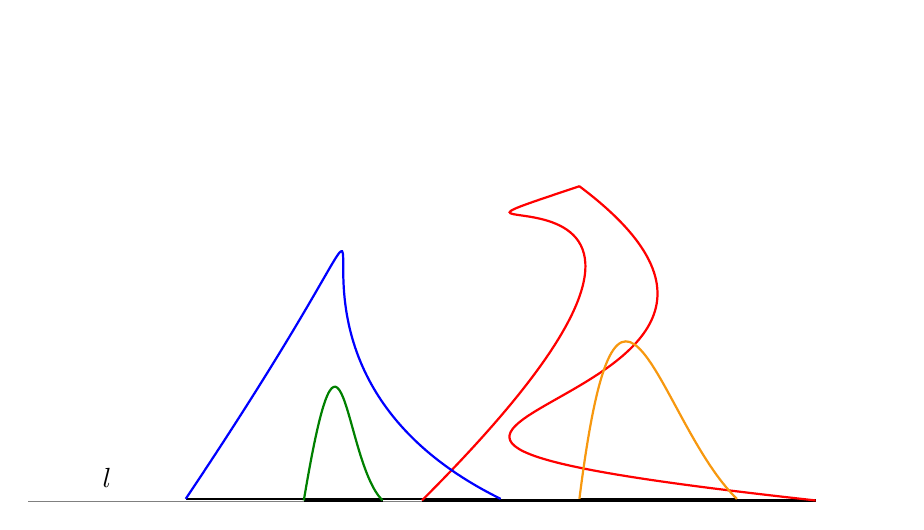
\begin{tikzpicture}
		\draw[color = gray] (0,0) -- (10,0);
		\node at (1,.3) {$l$};
		
		\draw[color=black, thick] (5,.01) edge (10,.01);
		\draw[color=black, thick] (7,.03) edge (9,.03);
		\draw[color=black, thick] (2,.03) edge (6,.03);
		\draw[color=black, thick] (3.5,.01) edge (4.5,.01);
		
		\draw[color=Red, thick] (5, .01) .. controls (10,5) and (4,3) .. (7, 4);
		\draw[color=Red, thick] (7, 4) .. controls (11,1) and (1,1) .. (10, .01);
		\fill[color=Red] (7,4) circle[radius=.35pt];
		
		\draw[color=Green, thick] (3.5, .01) .. controls (4,3) and (4,.5) .. (4.5, .01);
		\draw[color=Blue, thick] (2, .03) .. controls (6,6) and (2,2) .. (6, .03);
		\draw[color=YellowOrange, thick] (7, .03) .. controls (7.5,4) and (8,1) .. (9, .03);
	\end{tikzpicture}
	\caption{An illustration to the possible relative positions of interval-filaments.}
	\label{filaments}
\end{figure}
	\chapter{Cliques and independent sets}

We will show the computational complexity of the following optimization problems:

\begin{itemize}[]
	\item \textbf{Clique}
	\item \textit{Input:} A graph $G$.
	\item \textit{Output:} $\omega(G)$.
\end{itemize}

and

\begin{itemize} []
	\item \textbf{Independent Set}
	\item \textit{Input:} A graph $G$.
	\item \textit{Output:} $\alpha(G)$.
\end{itemize}

and their weighted variants

\begin{itemize}[]
	\item \textbf{Weighted Clique}
	\item \textit{Input:} A graph $G$ and a non-negative weight function $w : V(G) \to R_0^+$.
	\item \textit{Output:} A clique $C \subseteq V(G)$ which maximizes $w(C) = \sum_{u \in C} w(u)$.
\end{itemize}

and

\begin{itemize}[]
	\item \textbf{Weighted Independent Set}
	\item \textit{Input:} A graph $G$ and a non-negative weight function $w : V(G) \to R_0^+$.
	\item \textit{Output:} An independent set $A \subseteq V(G)$ which maximizes $w(A) = \sum_{u \in A} w(u)$.
\end{itemize}

Our goal is to show that for many of the intersection-defined graph classes that we have seen so far, these problems can be solved in polynomial time. For the sake of brevity, we denote by $\omega_w(G)$ the maximum possible weight $w(C)$ over all cliques $C$ in $G$, and by $\alpha_w(G)$ the maximum possible weight $w(A)$ over all independent sets $A$ in $G$.

\section{Interval graphs}

\begin{thm}
	\textbf{Weighted Clique} can be solved in polynomial time for interval graphs.
\end{thm}

\begin{proof}
	Interval graphs have only linearly many maximal cliques. We look at all of them and compare
	their weights.
\end{proof}

\begin{thm}
	\textbf{Weighted Independent Set} can be solved in polynomial time for interval graphs.
\end{thm}

\begin{proof}
	Suppose we are given an interval intersection representation $\mathcal{R} = \{I_u = [l_u , r_u] : u \in V\}$ of	a graph $G = (V, E)$, equipped with a weight function $w$. We may assume that all endpoints of the intervals are different. Number the endpoints $P_1 , P_2 , \dots , P_{2n}$ so that $P_i < P_{i+1}$ for $i = 1, 2, \dots , 2n - 1$.	Use dynamic programming to compute $w_i$ which is defined as the maximum possible weight of an	independent set $A$ in $G$ such that $r_u < P_i$ for all $u \in A$. This can be computed as follows:
	
	\begin{algorithm}[!ht]
		\begin{algorithmic}[1]
			\State $w_i := 0$
			\For{$i := 1$ to $2n$}
				\If{$P_i$ is the left endpoint of an interval}
					\State $w_{i+1} := w_i$
				\Else
					\State let $u \in V$ be such that $r_u = P_i$ and let $j$ be such that $P_j = l_u$;
					\State set $w_{i+1} = \max \{w_j + w(u), w_i\}$
				\EndIf
			\EndFor
			\State \Return $w_{2n+1}$
		\end{algorithmic}
	\end{algorithm}
\end{proof}

\begin{cor}
	\textbf{Weighted Clique} and \textbf{Weighted Independent Set} can both be solved in polynomial	time on co-INT graphs.
\end{cor}

\section{Comparability graphs}

\begin{thm}
	\textbf{Weighted Clique} can be solved in polynomial time for comparability graphs.
\end{thm}

\begin{proof}
	Given a transitive orientation $\overrightarrow{E}$ of $G = (V, E)$, order the vertices linearly $V = \{v_1 , v_2 , \dots, v_n\}$ in a topological sorting according to $\overrightarrow{E}$ (i.e., $v_i v_j \in \overrightarrow{E}$ implies $i < j$). For each $i$, set $W_i = \{j : v_j v_i \in E\}$ and let $w_i$ be the maximum weight $w(C)$ over all cliques $C \subseteq W_i \cup \{v_i\}$. Note that if $w(v_i) > 0$, each clique attaining the maximum weight contains $v_i$, and we may consider without loss	of generality only the cliques that contain $v_i$ even if $w(v_i) = 0$. The values $w_i , i = 1, 2, \dots , n$ can be computed recursively as follows
	
	\begin{algorithm}[!ht]
		\begin{algorithmic}[1]
			\For{$i := 1$ to $n$}
				\State $w_i := \max_{j \in W_i} w_j + w(v_i)$
			\EndFor
		\end{algorithmic}
	\end{algorithm}
	
	and clearly $\omega_w(G) = max_{i=1}^n w_i$.
\end{proof}

\begin{thm}
	\textbf{Weighted Independent Set} can be solved in polynomial time for \\ comparability graphs.
\end{thm}

\begin{proof}
	Given a transitive orientation $\overrightarrow{E}$ of $G = (V, E)$, consider the partial order $P = (V, \overrightarrow{E})$ determined by this orientation. The weighted version of Dilworth theorem yields that $\alpha_w(P)$ is equal to the minimum cost of a flow in the network $N = (V \cup \{s, t\}, E \cup \{su, ut : u \in V\})$ with vertex demands $f(u) \geq w(u)$, and this can be computed in polynomial time by network flow algorithms.
\end{proof}

\begin{cor}
	\textbf{Weighted Clique} and \textbf{Weighted Independent Set} can both be solved in polynomial time on function (= co-comparability) graphs.
\end{cor}

\section{Interval-filament graphs}

In this section we show the strongest results. Note, however, that we need the input graph to be given with an interval-filament representation (or, equivalently, with a partition of its edge set satisfying the mixing property).

\begin{thm}
	\textbf{Weighted Clique} can be solved in polynomial time for interval-filament graphs, if an interval-filament representation is provided on the input.
\end{thm}

\begin{proof}
	
\end{proof}
	\chapter{Recognition of Chordal graphs}

It is not surprising that chordal graphs can be recognized in polynomial time. Just search for a simplicial vertex, delete it if you find one and proceed recursively, or quit and say that the input graph
is not chordal if it has no simplicial vertex. Checking a vertex for being simplicial requires checking at most $n^2$ pairs of vertices if they are adjacent, hence a simplicial vertex can be found in $O(n^3)$ steps. Thus chordality can be checked in time $O(n^4)$. However, even if the graph is dense, i.e., if it has $m = \Omega(n^2)$, this naive algorithm still takes $\Omega(m^2)$ time. With more care, one can test chordality in time linear in the number of edges by the following algorithm.

\begin{algorithm}[!ht]
	\caption{LexBFS}
	\begin{algorithmic}[1]
		\Require A graph $G = (V,E)$ with $n$ vertices.
		\State $T := \emptyset, w(x) := \emptyset$ $\forall x \in V$
		\For{$i:= n \dots 1$}
			\State let $u \in V \setminus T$ be a vertex with lexicographicly maximum $w(u)$
			\State set $\sigma(i) := u$
			\State $T := T \cup \{u\}$
			\For{$x \in N_G (u) \cap (V \setminus T)$}
				\State $w(x) := w(x) \cup \{i\}$
			\EndFor
		\EndFor
	\end{algorithmic}
\end{algorithm}

\begin{thm}
	If $G = (V, E)$ is chordal, then $\sigma(n), \sigma(n - 1), . . . , \sigma(1)$ is a PES \faDog.
\end{thm}

\begin{proof}
	Suppose $G$ is chordal but there exist indices $i < j < h$ such that $\sigma(i)\sigma(j) \in E, \sigma(i)\sigma(h) \in E$ while $\sigma(j)\sigma(h) \notin E$. Let $i_0 < i_1 < i_2$ be such a triple and such that $i_2$ is largest possible.
	
	Let $u_i = \sigma(i), i = 1, 2, \dots , n$ be the ordering output by the Algorithm. Consider the step of the LexBFS algorithm when $i_1$ was processed. At this moment, $i_2 \in w(u_{i_0})$ while $i_2 \notin w(u_{i_1})$. Thus $u_{i_0}$ and $u_{i_1}$ do not have the same weights, and since $u_{i_1}$ was chosen for $\sigma(i_1)$, we must have $w(u_{i_0}) <_{lex} w(u_{i_1})$. Hence there must be $i_3 > i_2$ such that $u_{i_1} u_{i_3} \in E$ and $u_{i_0} u_{i_3} \notin E$. Let us choose $i_3$ as the largest index with these properties. An edge between $u_{i_2}$ and $u_{i_3}$ would imply that $G[\{u_0 , u_1 , u_2 ,u-3 \}]$ would be isomorphic to $C_4$, which would contradict the assumption that $G$ is chordal, and thus we conclude that $u_{i_2} u_{i_3} \notin E$.
	
	The same argument can now be used for $i_2$ and $i_3$ and further on:
	
	\begin{claim}
		For every $k > 3$, there exists a sequence $i_0 < i_1 < \dots < i_k$ such that $\{u_{i_0} u_{u_1}\} \cup \{u_{i_j} u_{i_{j+2}} : j = 0, 1, 2, \dots, k - 2\}$ are the only edges of $G$ among these vertices.
	\end{claim}
	
	\begin{proof}[Proof of claim]
		We proceed by induction on $k$. We have just seen that such a sequence exists for $k = 4$. Since the sequence is constructed recursively, we will further assume that in each step we have chosen $i_k$ largest possible.
		
		For the induction step $k \to k + 1$, we observe that at the moment when $i_{k-1}$ was processed, $i_k$ was in $w(u_{k-2})$ but not in $w(u_{k-1})$. Since $u_{i_{k-1}}$ was chosen for $\sigma(i_{k-1})$, it must have been $w(u_{i_{k-1}}) >_{lex} w(u_{i_{k-2}})$, and so there must be an $i_{k+1} > i_k$ such that $u_{i_{k-1}} u_{i_{k+1}} \in E$ while $u_{i_{k-2}} u_{i_{k+1}} \notin E$ (recall that we choose $i_{k+1}$ maximum possible with this property). Suppose there is a $j$, $0 \leq j \leq k - 3$ such that $u_{i_j} u_{i_{k+1}} \in E$, and consider the largest possible such $j$. If $j = k - 3$, then both $u_{i_{k+1}}$ and $u_{i_{k-1}}$ are adjacent to $u_{i_{k-3}}$ and non-adjacent to $u_{i_{k-2}}$ and this contradicts the presumed choice of
		$i_{k-1} < i_{k+1}$ as the largest possible index of this property. If $j < k - 3$, then $i_j < i_{j+2} < i_{k+1}$ would be	a triple violating the PES condition (since $u_{i_j} u_{i_{j+2}}, u_{i_j} u_{i_{k+1}} \in E$ and $u_{i_{j+2}} u_{i_{k+1}} \notin E$) with $i_{k+1} > i_2$ contradicting the choice of $i_0 < i_1 < i_2$. Thus $u_{i_j} u_{i_{k+1}} \notin E$ for $j = 0, 1, \dots, k - 2$. If $u_{i_k} u_{i_{k+1}}$ were an edge, $G[\{u_{i_h} : h = 0, 1, \dots, k + 1\}]$ would be isomorphic to $C_{k+2}$, which is impossible as $G$ is assumed to be chordal. This concludes the proof of the Claim.
	\end{proof}
	
	Since $G$ is finite, the sequence of the properties guaranteed by the Claim cannot exist, e.g., for $k > n$. So no triple of indices $i < j < h$ violating the PES condition may exist.
\end{proof}

With a suitable data structure, the LexBFS algorithm can be implemented to run in time linear in the number $m$ of edges of the input graph (the point is that this algorithm processes every edge of the graph only once).

However, this is only one half of testing for chordality. The algorithm LexBFS outputs a linear ordering of the vertices of $G$, but we need to test this ordering if it is a PES or not. This can, fortunately, also be achieved in linear time.

\begin{algorithm}[!ht]
	\caption{TestPES \faDog}
	\begin{algorithmic}[1]
		\Require A graph $G = (V, E)$ with $n$ vertices, a linear ordering $\sigma(i) \in V, i = 1, 2, \dots, n$ of its vertices.
		\Ensure \textbf{YES} or \textbf{NO} if $\sigma(n), \sigma(n-1), \dots, \sigma(1)$ is a PES.
		\State $A(x) := \emptyset$ for all $x \in V$
		\For{$i := 1 \dots n-1$}
			\State $v:= \sigma(i)$
			\State $X:= \{x : x \in N_G (v) \land \sigma^{-1}(v) < \sigma^{-1}(x)\}$
			\If{$X \neq \emptyset$}
				\State $u := \min \sigma^{-1}(X)$
				\State $A(u) := A(u) \cup (X \setminus \{u\})$
			\EndIf
			\If{$A(v) \setminus N_G (v) \neq \emptyset$}
				\State \Return \textbf{NO}
			\EndIf
		\EndFor
		\State \Return \textbf{YES} \faDog
	\end{algorithmic}
\end{algorithm}

\begin{thm}
	Algorithm TestPES correctly answers if a linear ordering $\sigma(n), \sigma(n-1), \dots, \sigma(1)$ is a PES for $G$ or not and it can be implemented in time linear in $m$.
\end{thm}

\begin{proof}
	For each vertex $u \in V$, the set $A(u)$ contains vertices that should be neighbors of $u$ if the ordering is a PES. The point is that it is not necessary to put in $A(u)$ all neighbors, and thus the running time can be significantly reduced.
	
	\begin{claim}
		If $\sigma(n), \sigma(n-1), \dots, \sigma(1)$ is not a PES, then at least one violation gets detected.
	\end{claim}
	
	\begin{proof}[Proof of claim]
		Let $i < j < h$ be a violation (i.e., $\sigma(i)\sigma(j), \sigma(i)\sigma(h) \in E$, $\sigma(j)\sigma(h) \notin E$) such that the difference $j - i$ is minimum possible. Let $v = \sigma(i)$. Then $\sigma(j), \sigma(h) \in X$ when $v$ is processed by the algorithm. Suppose there is a $j' , i < j' < j$ such that $\sigma(j') \in X$. If $\sigma(j')\sigma(j) \notin E$, $i < j' < j$ is a violation with smaller difference $j' - i < j - i$. If $\sigma(j')\sigma(h) \notin E$, $i < j' < h$ is a violation with smaller difference $j' - i < j - i$. If both $\sigma(j')\sigma(j)$ and $\sigma(j')\sigma(h)$ are edges, $j' < j < h$ is a violation with smaller difference $j - j' < j - i$. Since all possibilities lead to contradictions, we conclude that $j = \min\{l : \sigma(l) \in X\}$ and $\sigma(h)$ is put into $A(\sigma(j))$ when $v$ is being processed. Thus the non-edge $\sigma(j)\sigma(h)$ gets detected when $u = \sigma(j)$ is processed (unless the algorithm quits even sooner).
	\end{proof}
\end{proof}

\begin{rem}
	Note that the correctness of Algorithm LexBFS implies that not only one can leave any simplicial vertex as the last one in a PES, but it is also true that any vertex of a chordal graph can be used as the first vertex in a PES.
\end{rem}
	\chapter{Recognition of Comparability graphs}

Recall that comparability graphs are exactly the transitively orientable graphs. And that a transitive orientation is a binary relation on the vertex set of the graph which is transitive and orients every edge of the graph in exactly one direction. In order to eventually construct such a relation, if it exists, we will examine partial orientations and relations with further useful properties. Throughout
this handout we assume that we are processing a given simple undirected graph $G = (V, E)$.

\begin{defn}
	A relation $M \subseteq V \times V$ is called
	
	\begin{itemize}
		\item \textbf{sensitive} if for every three vertices $x, y, z \in V$, it holds true that $(x, y) \in M, xz \in E, yz \notin E$ imply $(x, z) \in M$, and $(x, y) \in M$, $zy \in E$, $xz \notin E$ imply $(z, y) \in M$,
		\item \textbf{complete} if it is sensitive and transitive,
		\item \textbf{faithful} if for every two vertices $x, y \in V$, it holds true that $(x, y) \in M$ implies $xy \in E$, and
		\item \textbf{whole} if for every edge $xy \in E$, at least one of $(x, y), (y, x)$ is in $M$.
	\end{itemize}
\end{defn}

\begin{observ}
	Every faithful, transitive and whole relation is necessarily sensitive.
\end{observ}

\begin{proof}
	Suppose $x, y, z$ are such that $(x, y) \in M$, $xz \in E$ and $yz \notin E$. Since $M$ is whole, we have either $(x, z) \in M$ or $(z, x) \in M$. In the case of $(z, x) \in M$, transitivity of $M$ would imply $(z, y) \in M$,	what would be in contradiction with the assumed faithfulness of $M$. Hence it must be $(x, z) \in M$. The symmetric rule is proven analogously.
\end{proof}

\begin{observ}
	Every transitive and faithful relation is necessarily antisymmetric (because we only consider simple - and henceforth loopless - graphs). Therefore transitive \\ orientations of $G$ are exactly those relations that are transitive, whole and faithful, and these are exactly those relations that are complete, whole and faithful.
\end{observ}

\begin{observ}
	The intersection of sensitive (transitive, complete) relations is a sensitive (transitive, complete, respectively) relation.
\end{observ}

The last observation implies that closures are defined uniquely:

\begin{defn}
	Let $M \subseteq V \times V$ be a binary relation. The smallest relation which contains $M$ and which is sensitive (transitive, complete) is called the sensitive- (transitive-, complete-, respectively) closure of $M$ and is denoted by $\langle M \rangle_{S}$ ($\langle M \rangle_{T}$ , $\langle M \rangle$, respectively).
\end{defn}

\begin{lemma}
	For any binary relation $M \subseteq V \times V$, it is $\langle M \rangle_{} = \langle\langle M \rangle_{S}\rangle_{T}$.
	\label{lemma-1}
\end{lemma}

\begin{proof}
	It suffices to show that $\langle\langle M \rangle_{S}\rangle_{T}$ is sensitive. Suppose $x, y, z \in V$ are such that $(x, y) \in \langle\langle M \rangle_{S}\rangle_{T}, xz \in E, yz \notin E$. Then there is a sequence $x = x_1 , x_2 , \dots, x_k = y$ such that $x_i x_{i+1} \in \langle M \rangle_{S}$ for every $i = 1, 2, \dots, k-1$. Since $x_1 z \in E$ and $x_k z \notin E$, there is an index $i, 1 \leq i < k$ such that $x_i z \in E$ and $x_{i+1} z \notin E$. Then $(xi , z) \in \langle M \rangle_S$ (this follows from its sensitivity), and hence $(x, z) \in \langle\langle M \rangle_{S}\rangle_{T}$	follows from the sequence of arcs $(x_1 , x_2), (x_2 , x_3), \dots, (x_{i-1} , x_i), (x_i , z) \in \langle M \rangle_{S}$.
\end{proof}

\section{Blocks}

\begin{defn}
	A \textbf{block} is the sensitive closure $\langle(x, y)\rangle_S$ of a single arc $(x, y)$ such that $xy \in E$. A pathway of length $k - 1$ in $V \times V$ from $(a, b)$ to $(c, d)$ is a sequence $(x_i, y_i), i = 1, 2, \dots, k$ such that
	
	\begin{itemize}
		\item $(a,b) = (x_1, y_1), (c,d) = (x_k, y_k)$,
		\item for every $i = 1, 2, \dots, k, x_i y_i \in E$,
		\item for every $i = 1, 2, \dots, k - 1$, either $x_i = x_{i+1}$ and $y_i y_{i+1} \notin E$, or $y_i = y_{i+1}$ and $x_i x_{i+1} \notin E$.
	\end{itemize}
	
	The \textbf{distance} of $(a, b)$ and $(c, d)$ (denoted by $\text{dist}_\Gamma ((a, b), (c, d)))$ is the length of a shortest pathway	between $(a, b)$ and $(c, d)$.
\end{defn}

\begin{prop}
	Let $xy \in E$ be an edge of $G$. Then the block $\langle(x, y)\rangle_S$ determined by an orientation $(x, y)$ of $xy$ contains exactly those arcs $(u, v)$ that are connected by pathways from $(x, y)$ to $(u, v)$. For every $(u, v) \in \langle(x, y)\rangle_S$, this arc defines the same block, i.e., $\langle(x, y)\rangle_S = \langle(u, v)\rangle_S$.
\end{prop}

\begin{proof}
	Define the graph $\Gamma_G = ((V \times V ) \cap \{(x, y) : xy \in E\}, \{(x, y)(u, v) : (x = u, yv \notin E) \land (y = v, xu \notin E)\})$ that captures the sensitive-rule constellations. Then blocks are connected components	of $\Gamma_G$. The concatenation of pathways from $(x, y)$ to $(u, v)$ and from $(u, v)$ to $(s, t)$ is a pathway from $(x, y)$ to $(s, t)$. Hence $\langle(u, v)\rangle_S \subseteq \langle(x, y)\rangle_S$ for every $(u, v) \in \langle(x, y)\rangle_S$. Since a pathway from $(x, y)$ to $(u, v)$ traversed in the opposite way is a pathway from $(u, v)$ to $(x, y)$, we get $\langle(x, y)\rangle_S = \langle(u, v)\rangle_S$.
\end{proof}

\begin{cor}
	For an edge $xy \in E$, it is $\langle(y, x)\rangle_S = \langle(x, y)\rangle_{S}^{-1}$ and both $\langle(x, y)\rangle_S$ and $\langle(y, x)\rangle_S$ are faithful.
\end{cor}

\begin{lemma}
	Let $xy \in E$ be an edge of $G$. If the block $\langle(x, y)\rangle_S$ is antisymmetric, then it is also transitive, and hence $\langle(x, y)\rangle = \langle(x, y)\rangle_S$ is faithful and complete.
	\label{lemma-2}
\end{lemma}

\begin{proof}
	For the sake of brevity, denote $U = \langle(x, y)\rangle_S$. Suppose $U$ is not transitive, i.e., there exist vertices $a, b, c \in V$ such that $(a, b), (b, c) \in U$ and $(a, c) \notin U$. Since $U$ is faithful, $ab, bc \in E$. It follows from the Proposition above that $\langle(a, b)\rangle_S = U$, and hence there is a pathway from $(a, b)$ to $(b, c)$ in $G$. Let the choice of the transitivity violating triple $a, b, c$ be such that the distance of $(a, b)$ and $(b, c)$ is the smallest possible.
	
	If $ac$ were not an edge of $G$, sensitivity of $U$ would imply $(c, b) \in U$ and that would be a contradiction with the assumed antisymmetry of $U$. Thus $ac \in E$.
	
	Let $(a, b) = (x_1 , y_1), (x_2 , y_2), \dots, (x_k , y_k ) = (b, c)$ be a shortest pathway from $(a, b)$ to $(b, c)$ in $G$ and let $l$ be the largest index such that $y_l \neq c$. Note that $x_l = x_{l+1}$ and $y_i = c$ for all $i = l + 1, \dots, k$. Set $\alpha = x_l$ and $\beta = y_l$.
	
	\begin{claim}
		For every $i = l+1, \dots, k, ax_i \in E$.
	\end{claim}
	
	\begin{proof}[Proof of claim]
		If for any such $i$ were $ax_i \notin E$, the sensitivity rule applied to $a, x_i , y_i = c$ would imply $ac \in U$ and $a, b, c$ would not violate transitivity.
	\end{proof}
	
	\begin{claim}
		For every $i = l+1, \dots, k, (a, x_i) \in U$.
	\end{claim}
	
	\begin{proof}[Proof of claim]
		We know that $(a, x_k = b) \in U$ and applying the sensitivity rule backwards on triples $x_i , c, x_{i-1}$ for $i = k, k - 1, \dots, l + 1$, the claim is proven.
	\end{proof}
	
	\begin{claim}
		It is $(a, \beta = y_e) \notin U$.
	\end{claim}
	
	\begin{proof}[Proof of claim]
		If $(a, \beta)$ were in $U$, the sensitivity rule applied to $\beta, a, c$ would imply $(a, c) \in U$, what is assumed not be the case.
	\end{proof}
	
	Now $a, \alpha = x_l , \beta = y_l$ is another transitivity violating example (as we have proved that $(a, \alpha) \in U , (a, \beta) \notin U$, and $(\alpha, \beta) \in U$ since it is included in the pathway). The sequence $(a, \alpha), (a, x_{l+2}), \dots, (a, x_k = b), (x_2 , y_2 ), \dots, (x_l = \alpha, y_l = \beta)$ is a pathway from $(a, \alpha)$ to $(\alpha, \beta)$ of length $k - l-  1 + l - 1 = k - 2 < \text{dist}_\Gamma ((a, b), (b, c))$, contradicting the choice of $a, b, c$.
\end{proof}

\section{Structure of transitive orientations}

If $G$ allows a transitive orientation $T$, each edge $xy \in E$ must be oriented one way or the other, and hence $\langle(x, y)\rangle_S \subseteq T$ or $\langle(y, x)\rangle_S \subseteq T$. Thus $\langle(x, y)\rangle_S$ must be antisymmetric for every edge $xy \in E$. The goal of this section is to show that this obvious necessary condition is also sufficient.

\begin{thm}
	A graph $G$ is transitively orientable if and only if the block $\langle(x, y)\rangle_S$ is antisymmetric for every $xy \in E$.
	\label{thm-24}
\end{thm}

The proof of the Theorem will follow from the following Lemma \ref{lemma-3}, which will also serve as a tool for finding a transitive orientation, if one exists.

\begin{lemma}
	Let $M \subseteq V \times V$ be a faithful complete binary relation and let $xy \in E$ be an edge such that $\langle(x, y)\rangle_S$ is antisymmetric and $M \cap \{(x, y), (y, x)\} = \emptyset$. Then $\langle M \cup \{(x, y)\}\rangle$ is faithful.
	\label{lemma-3}
\end{lemma}

\begin{proof}
	Denote by $U = \langle(x, y)\rangle_S$. Then $U = \langle(x, y)\rangle$ follows from Lemma \ref{lemma-2}. Since $M \cap \{(x, y), (y, x)\} = \emptyset$, it follows from the structure of blocks that $M \cap (U \cup U^{-1}) = \emptyset$, and hence $\langle M \cup \{(x, y)\}\rangle_S = M \cup U$. Lemma \ref{lemma-1} then implies that $\langle M \cup \{(x, y)\}\rangle = \langle\langle M \cup \{(x, y)\}\rangle_S \rangle_T = \langle M \cup U \rangle_T$.
	
	Suppose for the contrary that $\langle M \cup U \rangle_T$ is not faithful. Then there exists a sequence of edges $x_1 x_2 , x_2 x_3 , \dots, x_{k-1} x_k$ such that $(x_i , x_{i+1}) \in M \cup U$ for all $i = 1, 2, \dots, k - 1$ and $x_1 x_k \notin E$. Since $x_2 x_1 \in E$ and $x_k x_1 \notin E$, there is a $j, 2 \leq j < k$ such that $x_j x_1 \in E$ and $x_{j+1} x_1 \notin E$. Sensitivity of $M \cup U$ then implies that $x_j x_1 \in M \cup U$ and $M \cup U$ contains a directed cycle.
	
	Let $C$ be a shortest cycle in $M \cup U$. Since both $M$ and $U$ are transitive, the arcs of $C$ alternatively come from $M$ and $U$. The length of $C$ is at least 4, because a cycle of length 2 would contradict the assumption that $M \cap U^{-1} = \emptyset$. No diagonal of $C$ belongs to $M \cup U$, since any such diagonal would create a shorter cycle. Finally, all diagonals of $C$ are edges of $G$, since otherwise the sensitivity of $M \cup U$ would imply that either some diagonal belongs to $M \cup U$, or some arc of the cycle belongs to $M \cap U^{-1}$.
	
	Let now $a, b, c, d$ be consecutive vertices of $C$ such that $(a, b), (c, d) \in U$ and $(b, c) \in M$. Let the choice of $C$ and of $a, b, c, d$ be such that $\text{dist}_\Gamma ((a, b), (c, d))$ is minimum possible among all such choices. Note again that we have already observed that $ac, bd, ad \in E$, $\{(a, c), (c, a), (b, d), (d, b), (a, d)\} \cap (M \cup U) = \emptyset$ and $(d, a) \notin U$.
	
	Consider a shortest pathway $(a, b) = (x_1 , y_1), (x_2 , y_2), \dots , (x_k , y_k) = (c, d)$. Let $l$ be the smallest
	index such that $y_l \neq b$ (i.e., $y_1 = y_2 = \dots = y_{l-1} = b, x_{l-1} = x_l and x_1 , x_2 , \dots , x_{l-1}$ are pair-wise
	different). Set $\alpha = x_l$ and $\beta = y_l$ . We proceed with a sequence of observations.

	\begin{claim}
		For every $i = 1, 2, \dots , l, x_i d \in E$.
	\end{claim}
	
	\begin{proof}[Proof of claim]
		If $x_i d$ were a non-edge for some $i$, sensitivity would imply $(d, b) \in U$.
	\end{proof}
	
	\begin{claim}
		For every $i = 1, 2, \dots , l, x_i c \in E$.
	\end{claim}
	
	\begin{proof}[Proof of claim]
		If $x_j c$ were a non-edge for some $j$, sensitivity of $U$ would imply $(x_j , d) \in U$, and hence $(x_i , d) \in U$ for all $i = 1, 2, \dots , l$. Thus $(a, d) \in U$, contradicting the assumption.
	\end{proof}
	
	\begin{claim}
		It is $c\beta \in E$.
	\end{claim}
	
	\begin{proof}[Proof of claim]
		Otherwise sensitivity applied to $c, \alpha = x_l , \beta = y_l$ would imply $(\alpha, c) \in U$, and hence $(x_i , c) \in U$ for all $i = 1, 2, \dots , l$, and thus $(a, c) \in U$.
	\end{proof}
	
	\begin{claim}
		Now $(\beta, c) \in M$ follows from sensitivity of $M$ applied to $b, c, \beta$.
	\end{claim}
	
	\begin{claim}
		For every $i = 1, 2, \dots , l, x_i \beta \in E$.
	\end{claim}
	
	\begin{proof}[Proof of claim]
		If $x_j \beta$ were a non-edge for some $j$, sensitivity of $M$ would imply $(x_j , c) \in M$, hence we would get $(x_i , c) \in M$ for all $i = 1, 2, \dots , l$, and also $(a, c) \in M$.
	\end{proof}
	
	\begin{claim}
		Sensitivity of $U$ implies that $(x_i , \beta) \in U$ for all $i = 1, 2, \dots , l$, and hence also $(a, \beta) \in U$.
	\end{claim}

	Now we see that $a, \beta, c, d, \dots$ is a directed cycle in $M \cup U$ of the same length as $C$, while $\text{dist}_\Gamma ((a, \beta), (c, d)) \leq l - 2 + k - l = k - 2 < k - 1 = \text{dist}_\Gamma ((a, b), (c, d))$ since $(x_1 , \beta), (x_2 , \beta), \dots , (x_{l-1} , \beta), (x_{l+1} , y_{l+1}), \dots , (x_k , y_k )$ is a pathway from $(a, \beta)$ to $(c, d)$. This is the desired contradiction.
\end{proof}

\begin{proof}[Proof of Theorem \ref{thm-24}]
	We have already seen that if $G$ is transitively orientable, each block must be asymmetric.
	
	For the opposite implication, suppose that $G$ is such that each block $\langle(x, y)\rangle_S$, $xy \in E$, is asymmetric and suppose that $M \subseteq V \times V$ is a largest possible complete and faithful binary relation on $V$. If $M$ is not whole, there is an edge $xy \in E$ which is not oriented by $M$, i.e., $M \cap \{(x, y), (y, x)\} = \emptyset$. Lemma \ref{lemma-3} implies that $\langle M \cup \{(x, y)\}\rangle$ is a faithful complete relation, and it is clearly a strict superset of $M$. That would contradict the choice of $M$. Hence $M$ is whole, and thus a transitive orientation of $G$.
\end{proof}

\section{Algorithmic aspects}

Lemmas 2 and 3 also provide the correctness argument for a polynomial time algorithm for deciding if a graph is transitively orientable, and constructing such an orientation, if one exists.

\begin{algorithm}[!ht]
	\caption{Transitive Orientation}
	\begin{algorithmic}[1]
		\Require A graph $G = (V,E)$.
		\State $M := \emptyset$
		\While{$M$ is not whole}
			\State let $xy \in E$ be such that $M \cap \{(x,y), (y,x)\} = \emptyset$
			\State construct $U = \langle (x,y) \rangle_S$
			\If{$U$ is not antisymmetric}
				\State \Return "$G$ is not transitively orientable"
			\Else
				\State $M := \langle M \cup U \rangle_T$
			\EndIf
		\EndWhile
		\State \Return "$G$ is transitively orientable by $M$"
	\end{algorithmic}
\end{algorithm}
	\chapter{Visibility and contact representations of planar graphs}

\section{$s-t$ numbering}

\begin{defn}
	An $s - t$ numbering (also called a bipolar orientation) of a graph is an acyclic orientation of its edges which has exactly one source (a vertex with no in-coming arcs) and exactly one sink (a vertex with no out-going arcs).
\end{defn}

\begin{prop}
	Every vertex 2-connected graph has an $s - t$ numbering.
\end{prop}

\begin{proof}
	By induction on adding ears, using the Ear Decomposition Lemma. Given the starting cycle, choose two distinct vertices on it (to be the source and the sink) and orient the cycle as two directed paths from the source to the sink. The loop invariant will be that every vertex lies on a directed path from the source to the sink. When adding an ear, orient it in the direction from the source to the sink if both end-vertices of the ear lie on the same path from the source to the sink. If the end-vertices of the ear lie on different paths from the source to the sink, the ear may be oriented either way (but all of its edges in the same direction).
\end{proof}

\begin{thm}
	Every vertex 2-connected plane graph has an $s - t$ numbering and a noncrossing planar drawing such that
	
	\begin{enumerate}[i]
		\item every edge is drawn as a $y$-monotone curve (i.e., every horizontal line crosses the drawing of the edge in at most one point), and
		\item the drawing of every edge is oriented upward in the $s - t$ numbering.
	\end{enumerate}
	\label{thm-1}
\end{thm}

This $s - t$ numbering and a corresponding planar drawing can be constructed in polynomial time.

\begin{comm}
	By saying a plane graph it is meant a planar graph with a given noncrossing drawing in the plane, and it is understood that only drawings which are homeomorphic to the given one are considered, including the choice of the outerface.
\end{comm}

\begin{proof}
	By Ear Decomposition Lemma, the given graph $G$ can be constructed from the cycle bounding its outerface by adding ears. Choose two distinct vertices, say $a$ and $b$, on this cycle, place them in the plane so that they have different $y$-coordinates, the coordinate of a being smaller than the coordinate of $b$, orient the two $a - b$ paths forming the cycle from $a$ to $b$ and draw them as $y$-monotone paths from (the drawing of) a to (the drawing of) $b$.
	
	Then continue adding the ears, orienting their edges and adding them to the drawing constructed while keeping the following loop invariant -- the drawing is homeomorphic to the so far constructed part of $G$, it satisfies i) and ii), all vertices have distinct $y$-coordinates, and each face is bounded by two upward oriented paths connecting its vertices with the lowest and the highest $y$-coordinates (we will refer to these paths as the \textit{left} one and the \textit{right} one). Note that i) and ii) together imply that the drawing of any directed path is $y$-monotone.
	
	When an ear is added, it is added inside a face of the so far constructed part of $G$. Direct the edges of the ear in the direction from the vertex with the lower $y$-coordinate to the vertex with the higher one (the end-vertices of the ear belong to the so far constructed part of $G$ and so they have already been drawn). If the end-vertices belong to the same bounding path (the left one or the right one) of the face they should be draw in, draw the ear as a $y$-monotone curve contouring the bounding path. If the end-vertices belong to different bounding paths, draw the ear as a $y$-monotone curve that contours the path which contains the lower endpoint and traverse the face to the other endpoint almost horizontally close to the $y$-coordinate of this other endpoint, in order to avoid crossings with other edges. It is easy to check that the loop invariant of the construction is fulfilled.
\end{proof}

\begin{figure}[!ht]\centering
	\begin{subfigure}{0.45\textwidth}\centering
		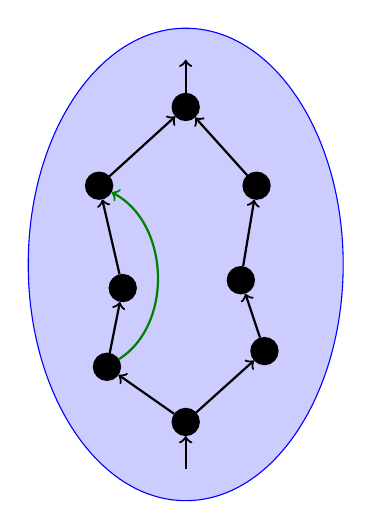
\begin{tikzpicture}[main/.style = {draw, circle, thick, fill}]
			% Draw ellipsoid
			\draw[blue, fill=blue!20] (0,0) ellipse (2 and 3);
			\node[main] (1) at (0,-2) {};
			\node[main] (2) at (-1,-1.3) {};
			\node[main] (3) at (1,-1.1) {};
			\node[main] (4) at (-0.8,-0.3) {};
			\node[main] (5) at (0.7,-0.2) {};
			\node[main] (6) at (-1.1,1) {};
			\node[main] (7) at (0.9,1) {};
			\node[main] (8) at (0,2) {};
			
			\draw[->, thick] (1) edge (2);
			\draw[->, thick] (1) edge (3);
			\draw[->, thick] (2) edge (4);
			\draw[->, thick] (3) edge (5);
			\draw[->, thick] (4) edge (6);
			\draw[->, thick] (5) edge (7);
			\draw[->, thick] (6) edge (8);
			\draw[->, thick] (7) edge (8);
			
			\draw[->, thick] (0, -2.6) -- (1);
			\draw[->, thick] (8) -- (0, 2.6);
			
			\draw[->, thick, color=Green, bend right = 60] (2) edge (6);
		\end{tikzpicture}
	\end{subfigure}
	\begin{subfigure}{0.45\textwidth}\centering
		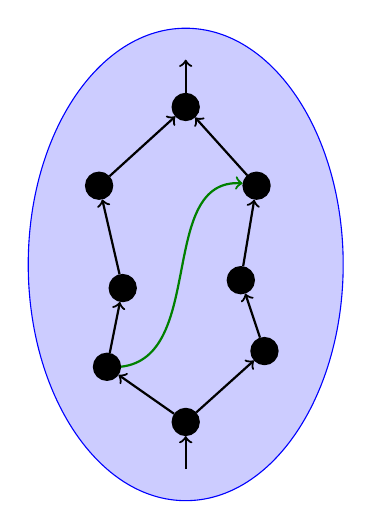
\begin{tikzpicture}[main/.style = {draw, circle, thick, fill}]
			% Draw ellipsoid
			\draw[blue, fill=blue!20] (0,0) ellipse (2 and 3);
			\node[main] (1) at (0,-2) {};
			\node[main] (2) at (-1,-1.3) {};
			\node[main] (3) at (1,-1.1) {};
			\node[main] (4) at (-0.8,-0.3) {};
			\node[main] (5) at (0.7,-0.2) {};
			\node[main] (6) at (-1.1,1) {};
			\node[main] (7) at (0.9,1) {};
			\node[main] (8) at (0,2) {};
			
			\draw[->, thick] (1) edge (2);
			\draw[->, thick] (1) edge (3);
			\draw[->, thick] (2) edge (4);
			\draw[->, thick] (3) edge (5);
			\draw[->, thick] (4) edge (6);
			\draw[->, thick] (5) edge (7);
			\draw[->, thick] (6) edge (8);
			\draw[->, thick] (7) edge (8);
			
			\draw[->, thick] (0, -2.6) -- (1);
			\draw[->, thick] (8) -- (0, 2.6);
			
			\draw[->, thick, color=Green, bend right, out=-50, in=120] (2) edge (7);
		\end{tikzpicture}
	\end{subfigure}
	\caption{An illustration to adding an ear in the construction of an $s-t$ numbering and a corresponding upward drawing.}
\end{figure}

\section{Rectangle visibility representations of planar \\ graphs}

\begin{defn}
	A \textbf{rectangle visibility representation} of a plane graph $G$ is an arrangement of disjoint axes-aligned rectangles in the plane such that the (unions of) horizontal sides of the rectangles correspond to the vertices of $G$, the (unions of) vertical sides to the faces of $G$, and each rectangle corresponds to the edge joining the vertices containing the upper and lower sides of the rectangle, and at the same time to the dual edge joining the faces corresponding to the left and right sides of the rectangle.
\end{defn}

\begin{comm}
	In this section we allow multiple edges without explicitly talking about \\ multigraphs. Moreover, we artificially choose two vertices on the boundary of the outerface and divide the outerface into two faces by "infinite" dummy edges starting in these points.
\end{comm}

\begin{figure}[!ht]\centering
	\begin{subfigure}{0.6\textwidth}\centering
		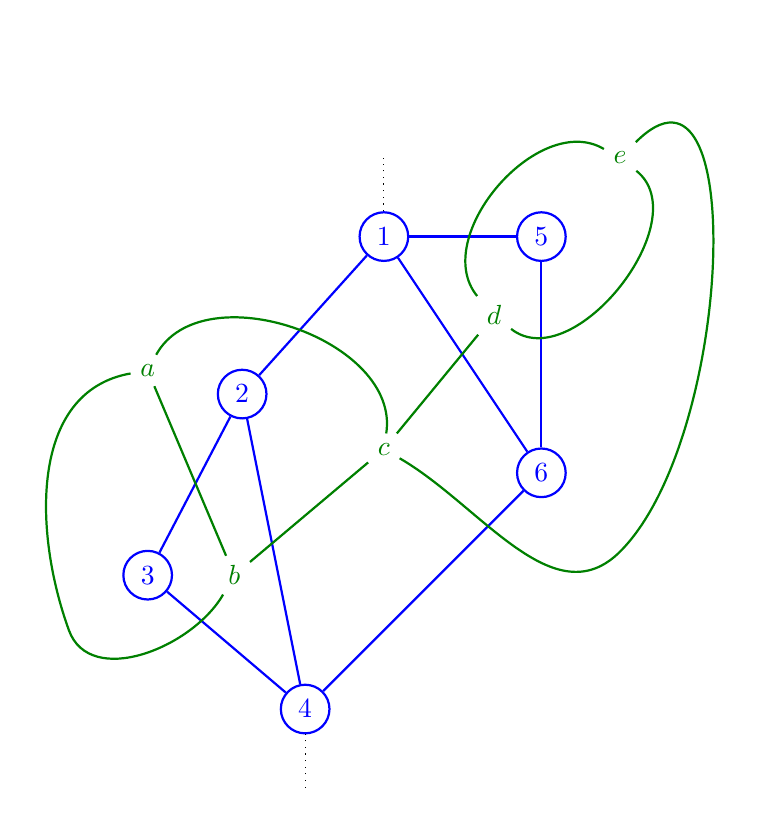
\begin{tikzpicture}[main/.style = {draw, circle, thick, color = Blue}]
			\node[main] (4) at (0,0) {4};
			\node[main] (3) at (-2,1.7) {3};
			\node[main] (6) at (3,3) {6};
			\node[main] (2) at (-0.8,4) {2};
			\node[main] (5) at (3,6) {5};
			\node[main] (1) at (1,6) {1};
			\node[color=Green] (b) at (-0.9, 1.7) {$b$};
			\node[color=Green] (a) at (-2, 4.3) {$a$};
			\node[color=Green] (c) at (1, 3.3) {$c$};
			\node[color=Green] (d) at (2.4, 5) {$d$};
			\node[color=Green] (e) at (4, 7) {$e$};
			\draw[thick, color=Blue] (4) edge (3);
			\draw[thick, color=Blue] (4) edge (2);
			\draw[thick, color=Blue] (4) edge (6);
			\draw[thick, color=Blue] (5) edge (6);
			\draw[thick, color=Blue] (6) edge (1);
			\draw[thick, color=Blue] (2) edge (1);
			\draw[thick, color=Blue] (1) edge (5);
			\draw[thick, color=Blue] (2) edge (3);
			\draw[dotted] (0, -1) -- (4);
			\draw[dotted] (1) -- (1, 7);
			\draw[thick, color=Green] (b) edge (c);
			\draw[thick, color=Green] (d) edge (c);
			\draw[thick, color=Green] (b) edge (a);
			
			\coordinate (6') at (4,2);
			\coordinate (3') at (-3, 1);
			
			\draw[thick, color=Green] (b) to[out = 240, in = -70] (3') to[out = 110, in = 190] (a);
			\draw[thick, color=Green, bend left = 80] (a) edge (c);
			\draw[thick, color=Green] (e) to[out = 45, in = 45] (6') to[out = -135, in = -30] (c);
			\draw[thick, color=Green, bend left = 80] (d) edge (e);
			\draw[thick, color=Green, bend right = 90] (d) edge (e);
		\end{tikzpicture}
	\end{subfigure}
	\begin{subfigure}{0.35\textwidth}\centering
		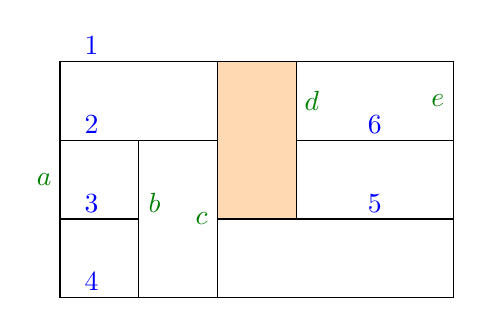
\begin{tikzpicture}
			\draw[black] (0,0) rectangle (1,1);
			\draw[black] (0,1) rectangle (1,2);
			\draw[black] (1,0) rectangle (2,2);
			\draw[black] (2,0) rectangle (5,1);
			\draw[black] (0,2) rectangle (2,3);
			\draw[black, fill=orange!30] (2,1) rectangle (3,3);
			\draw[black] (3,1) rectangle (5,2);
			\draw[black] (3,2) rectangle (5,3);
			\node[Blue] at (0.4, 3.2) {1};
			\node[Blue] at (0.4, 2.2) {2};
			\node[Blue] at (0.4, 1.2) {3};
			\node[Blue] at (0.4, 0.2) {4};
			\node[Green] at (-0.2, 1.5) {$a$};
			\node[Green] at (1.2, 1.2) {$b$};
			\node[Green] at (1.8, 1) {$c$};
			\node[Blue] at (4, 1.2) {5};
			\node[Blue] at (4, 2.2) {6};
			\node[Green] at (3.2, 2.5) {$d$};
			\node[Green] at (4.8, 2.5) {$e$};
		\end{tikzpicture}
	\end{subfigure}
	\caption{An example of a rectangle visibility representation of a planar graph. The highlighted rectangle in the representation corresponds to the primal edge 13 and dual edge $cd$.}
\end{figure}

\begin{thm}
	Every planar vertex 2-connected graph has a rectangle visibility \\ representation.
	\label{thm-2}
\end{thm}

\begin{proof}
	We in fact describe an algorithm how such a representation can be constructed. The bonus is that the construction runs in polynomial time.
\end{proof}

\begin{algorithm}[!ht]
	\caption{RectangleVisibilityRep}
	\begin{algorithmic}[1]
		\Require A planar graph $G$.
		\State Construct an $s - t$ numbering and a corresponding upward planar drawing as in Theorem \ref{thm-1}.
		\State Number the vertices as $1, \dots, n$ according to their $y$-coordinates (1 is the lowest vertex, $n$ is the highest one).
		\State Add a dummy arc from 1 to $n$ drawn to the right of the drawing of $G$, denote by $G'$ the resulting graph.
		\State Construct the dual graph $G^\ast$ to $G'$, and orient its edges so that each edge of $G$ is crossed by its dual edge from left to right, while the added dummy edge is crossed from right to left. Let $n^\ast$ be the number of vertices of $G^\ast$.
		\State Consider a topological sorting of the vertices of $G^\ast$ and name them $A, B, \dots$ according to this sorting.
		\State Take a grid of size $n \times n^\ast$. For a vertex $i$ of $G$, let $\alpha(\beta)$ be the face incident with $i$ with the lowest (highest, respectively) name in the topological sorting of $G^\ast$. Represent $i$ by a horizontal segment on the $i$-th line, starting at the vertical line $\alpha$ and ending on the vertical line $\beta$. For a face $\alpha$ of the drawing of $G'$ (i.e., a vertex of the dual graph $G^\ast$), let $i$ be its lowest vertex and $j$ its highest vertex (with respect to the topological sorting of $G$). Represent $\alpha$ by a segment on the vertical line $\alpha$, starting on the $i$-th horizontal line and ending on the $j$-th one.
		\State \Return this representation.
	\end{algorithmic}
\end{algorithm}

It is, however, necessary to prove that this Algorithm really outputs a rectangle visibility representation of $G$. This is done via a series of claims. The first ones talk about the upward drawing of $G$ constructed in Step 1 and the dual graph $G^\ast$ and its drawing inherited from the drawing of $G$.

\begin{claim}
	Vertex number 1 and vertex number $n$ are both on the boundary of the outerface of $G$ (and also of $G'$). The face that gets the name $A$ is the unbounded face and the face with the highest name, say $Z$, is the other face incident with the dummy edge $1n$.
\end{claim}

\begin{claim}
	The orientation of $G^\ast$ described in Step 4 is acyclic and $A$ is its only source and $Z$ is its only sink. Hence it is indeed an $s - t$ numbering of $G^\ast$. To see this, note first that the edge $AZ$ which crosses the dummy edge $1n$ cannot be involved in any directed cycle, as $A$ is a source and $Z$ is a sink in $G^\ast$. Next observe that a clock-wise oriented cycle in $G^\ast$ would bound a region with at least one vertex of $G$ inside and all edges of $G$ crossing this cycle would be oriented from inside towards the outside of this region, hence, there would necessarily be a source of $G$ in this region, and this would be different from the vertex $1$. Similarly, a counter-clock-wise oriented cycle in $G^\ast$ would bound a region that would contain a sink different from $n$. This would be a contradiction with the assumption that we were working with an $s - t$-numbering of $G$. Finally, a source different from $A$ (a sink different from $Z$) in $G^\ast$ would yield a directed cycle on the boundary of this face of $G$. A contradiction again.
\end{claim}

\begin{claim}
	The boundary of every face $\alpha$ of $G$ consists of two directed paths, the left one and the right one, both connecting the vertex of the lowest number to the vertex of the highest number among the vertices of this face. We have seen this in the proof of Theorem \ref{thm-1}.
\end{claim}

\begin{claim}
	For every vertex $i$ of $G, i \neq 1, n$, the faces incident with $i$ induce two directed paths in $G^\ast$,
	both connecting the face to the left of $i$ to the face lying to the right of $i$, one of the paths passing
	through the faces for which $i$ is their topmost vertex, the other one passing through the faces for which
	$i$ is their lowest vertex. See Fig. \ref{fig-3} right.
\end{claim}

\begin{figure}[!ht]
	\begin{subfigure}{0.45\textwidth}\centering
		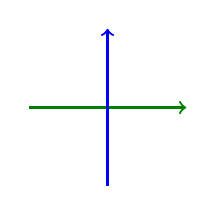
\begin{tikzpicture}
			\draw[->, color=Green, thick] (0,0) -- (2,0);
			\draw[->, color=Blue, thick] (1, -1) -- (1, 1);
		\end{tikzpicture}
	\end{subfigure}
	\begin{subfigure}{0.45\textwidth}\centering
		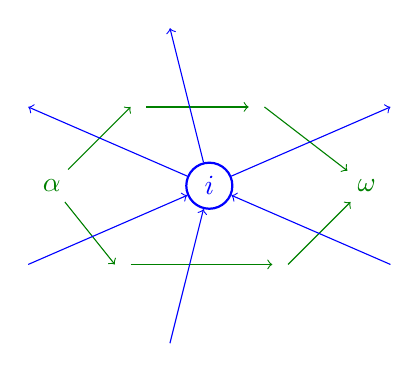
\begin{tikzpicture}
			\node[draw, circle, Blue, thick] (i) at (0,0) {$i$};
			\node[Green, thick] (a) at (-2, 0) {$\alpha$};
			\node[Green, thick] (w) at (2,0) {$\omega$};
			\draw[->, Green] (a) -- (-1, 1);
			\draw[->, Green] (-0.8,1) -- (0.5, 1);
			\draw[->, Green] (0.7, 1) -- (w);
			\draw[->, Green] (a) -- (-1.2, -1);
			\draw[->, Green] (-1, -1) -- (0.8, -1);
			\draw[->, Green] (1, -1) -- (w);
			\draw[->, Blue] (i) -- (-0.5, 2);
			\draw[->, Blue] (-0.5, -2) -- (i);
			\draw[->, Blue] (i) -- (-2.3, 1);
			\draw[->, Blue] (-2.3, -1) -- (i);
			\draw[->, Blue] (i) -- (2.3, 1);
			\draw[->, Blue] (2.3, -1) -- (i);
		\end{tikzpicture}
	\end{subfigure}
	\caption{Orientation of the dual edges (left). An example to the statement of Claim 4 (right).}
	\label{fig-3}
\end{figure}

In the next claims we prove that the collection of segments constructed in Step 6 defines a rectangle visibility representation of $G$.

\begin{claim}
	Let $i$ be a vertex of $G, i \neq 1, n$. Let $\alpha$ and $\omega$ be the faces to the left and to the right of $i$, respectively. Then the (horizontal) segment $i$ touches the vertical segment for $\alpha$ from the right, it touches the vertical segment for $\beta$ from the left, it is touched by the segments representing the faces lying on the upper path from $\alpha$ to $\beta$ in $G^\ast$ from above, and it is touched by the faces lying on the lower path from $\alpha$ to $\beta$ in $G^\ast$ from below. The segment representing vertex $1$ spans the whole range from $A$ to $Z$ and is only touched by vertical segments from above, while the segment representing $n$ is only touched by vertical segments from below, and also spans the whole range from $A$ to $Z$.
	\label{claim-5}
\end{claim}

\begin{claim}
	Let $\alpha$ be an inner face of $G$, i.e., a face not incident with the dummy edge $1n$. The vertical segment representing $\alpha$ touches the horizontal segment representing its lowest vertex from above, it touches the segment representing its topmost vertex from below, it is touched by the segments representing the vertices on the left boundary path of $\alpha$ from the left and it is touched by the segments representing the vertices on the right boundary path of $\alpha$ from the right. The segment representing $A$ is touched only from right, while the segment representing $Z$ is touched only from left, always by the appropriate horizontal segments.
	\label{claim-6}
\end{claim}

\begin{figure}[!ht]
	\begin{subfigure}{.25\textwidth}\centering
		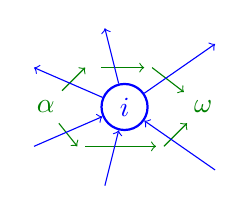
\begin{tikzpicture}
			\node[draw, circle, Blue, thick] (i) at (0,0) {$i$};
			\node[Green, thick] (a) at (-1, 0) {$\alpha$};
			\node[Green, thick] (w) at (1,0) {$\omega$};
			\draw[->, Green] (a) -- (-0.5, 0.5);
			\draw[->, Green] (-0.3,0.5) -- (0.25, 0.5);
			\draw[->, Green] (0.35, .5) -- (w);
			\draw[->, Green] (a) -- (-.6, -.5);
			\draw[->, Green] (-.5, -.5) -- (0.4, -.5);
			\draw[->, Green] (.5, -.5) -- (w);
			\draw[->, Blue] (i) -- (-0.25, 1);
			\draw[->, Blue] (-0.25, -1) -- (i);
			\draw[->, Blue] (i) -- (-1.15, .5);
			\draw[->, Blue] (-1.15, -.5) -- (i);
			\draw[->, Blue] (i) -- (1.15, .8);
			\draw[->, Blue] (1.15, -.8) -- (i);
		\end{tikzpicture}
	\end{subfigure}
	\begin{subfigure}{.2\textwidth}\centering
		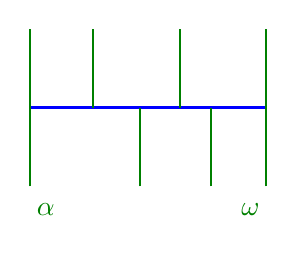
\begin{tikzpicture}
			\draw[thick, Blue] (0,0) -- (3,0);
			\draw[thick, Green] (0,-1) -- (0,1);
			\draw[thick, Green] (3,-1) -- (3,1);
			\draw[thick, Green] (.8,0) -- (.8,1);
			\draw[thick, Green] (1.9,0) -- (1.9,1);
			\draw[thick, Green] (1.4,-1) -- (1.4,0);
			\draw[thick, Green] (2.3,-1) -- (2.3,0);
			\node[Green] at (.2, -1.3) {$\alpha$};
			\node[Green] at (2.8, -1.3) {$\omega$};
		\end{tikzpicture}
	\end{subfigure}
	\begin{subfigure}{.25\textwidth}\centering
		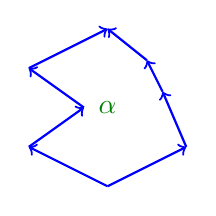
\begin{tikzpicture}
			\draw[->, thick, Blue] (0,0) -- (-1, .5);
			\draw[->, thick, Blue] (-1, .5) -- (-.3, 1);
			\draw[->, thick, Blue] (-.3, 1) -- (-1, 1.5);
			\draw[->, thick, Blue] (-1, 1.5) -- (0, 2);
			\draw[->, thick, Blue] (0,0) -- (1, .5);
			\draw[->, thick, Blue] (1, .5) -- (.7, 1.2);
			\draw[->, thick, Blue] (.7, 1.2) -- (.5, 1.6);
			\draw[->, thick, Blue] (.5, 1.6) -- (0,2);
			\node[Green, thick] at (0,1) {$\alpha$};
		\end{tikzpicture}
	\end{subfigure}
	\begin{subfigure}{.2\textwidth}\centering
		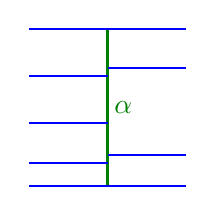
\begin{tikzpicture}
			\draw[Green, thick] (0,0) -- (0,2);
			\draw[Blue, thick] (-1,0) -- (1,0);
			\draw[Blue, thick] (-1,2) -- (1,2);
			\draw[Blue, thick] (-1,.3) -- (0,.3);
			\draw[Blue, thick] (-1,.8) -- (0,.8);
			\draw[Blue, thick] (-1,1.4) -- (0,1.4);
			\draw[Blue, thick] (0,.4) -- (1,.4);
			\draw[Blue, thick] (0,1.5) -- (1,1.5);
			\node[Green, thick] at (0.2, 1) {$\alpha$};
		\end{tikzpicture}
	\end{subfigure}
	\caption{Illustration to Claims \ref{claim-5} and \ref{claim-6}.}
\end{figure}

\begin{claim}
	For every edge $ij$ of $G$, let $\alpha\beta$ be its dual edge. Then the segments representing $i, j, \alpha$ and $\beta$ bound a rectangle in the representation.
	\label{claim-7}
\end{claim}

\begin{claim}
	No two segments constructed in Step 6 cross each other. For suppose segment $j$ crosses segment $\alpha$. By the way the segments are constructed, this means that there exist vertices $i, k, i < j < k$, and $\beta, \gamma, \beta < \alpha < \gamma$, such that $i$ is the lowest and $k$ the topmost vertex of face $\alpha$ and $\beta$ is the left and $\gamma$ the right face incident with $j$. Consider the upward drawing of $G$ and the horizontal stripe of vertices with their $y$-coordinates between $i$ and $k$. The face $\alpha$ spans this stripe from its bottom to its top lines, and thus it lies either to the left or to the right of vertex $i$. Suppose it is to the left. The horizontal ray starting in vertex $i$ and pointing to the left passes first through the face $\beta$ and then crosses several faces until it finally crosses $\alpha$. Since all edges of $G$ it crosses on this way are directed upward, these faces form a path directed from $\alpha$ to $\beta$ in $G^\ast$, which means that $\alpha < \beta$ in the topological sorting of $G^\ast$. Which is a contradiction.
	\label{claim-8}
\end{claim}

\begin{figure}
	\begin{subfigure}{.45\textwidth}\centering
		\begin{tikzpicture}
			\draw[thick, Green] (0,0) -- (0,3);
			\draw[thick, Blue] (-1.5,1.5) -- (1.5, 1.5);
			\draw[dotted] (-1.5, -.2) -- (-1.5, 3.2);
			\draw[dotted] (1.5, -.2) -- (1.5, 3.2);
			\draw[dotted] (-1.7, 0) -- (1.7, 0);
			\draw[dotted] (-1.7, 3) -- (1.7, 3);
			
			\node[Green] at (.3, .2) {$\alpha$};
			\node[Blue] at (1.2, 1.8) {$j$};
			\node[Blue] at (1.9, 0) {$i$};
			\node[Blue] at (1.9, 3) {$k$};
			\node[Green] at (-1.2, -.3) {$\beta$};
			\node[Green] at (1.2, -.3) {$\gamma$};
		\end{tikzpicture}
	\end{subfigure}
	\begin{subfigure}{.45\textwidth}\centering
		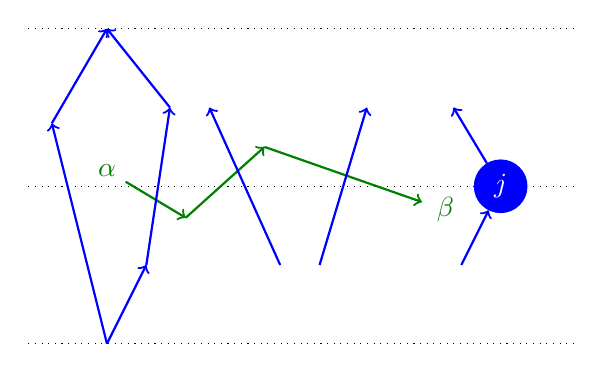
\begin{tikzpicture}
			\draw[dotted] (0,0) -- (7,0);
			\draw[dotted] (0,2) -- (7,2);
			\draw[dotted] (0,-2) -- (7,-2);
			\node[Green] (a) at (1, 0.2) {$\alpha$};
			\draw[->, thick, Green] (a) -- (2, -.4);
			\draw[->, thick, Green] (2, -.4) -- (3, .5);
			\draw[->, thick, Green] (3, .5) -- (5, -.2);
			\node[Green] (b) at (5.3, -.3) {$\beta$};
			\node[draw, circle, Blue, fill] (j) at (6, 0) {\textcolor{white}{$j$}};
			\draw[->, Blue, thick] (5.5, -1) -- (j);
			\draw[->, Blue, thick] (j) -- (5.4, 1);
			\draw[->, thick, Blue] (3.7, -1) -- (4.3,1);
			\draw[->, thick, Blue] (3.2, -1) -- (2.3,1);
			\draw[->, thick, Blue] (1.5, -1) -- (1.8,1);
			\draw[->, thick, Blue] (1,-2) -- (1.5, -1);
			\draw[->, thick, Blue] (1.8, 1) -- (1,2);
			\draw[->, thick, Blue] (1,-2) -- (.3, .8);
			\draw[->, thick, Blue] (.3, .8) -- (1,2);
		\end{tikzpicture}
	\end{subfigure}
	\caption{An illustration to Claim \ref{claim-8}.}
\end{figure}

\begin{claim}
	The rectangles from Claim \ref{claim-7} are disjoint and fill in the base rectangle formed by segments $A, Z, 1, n$. This now follows from the previous claims. And this means that we have indeed constructed a rectangle visibility representation of $G$.
\end{claim}

\begin{figure}[!ht]
	\begin{subfigure}{0.53\textwidth}\centering
		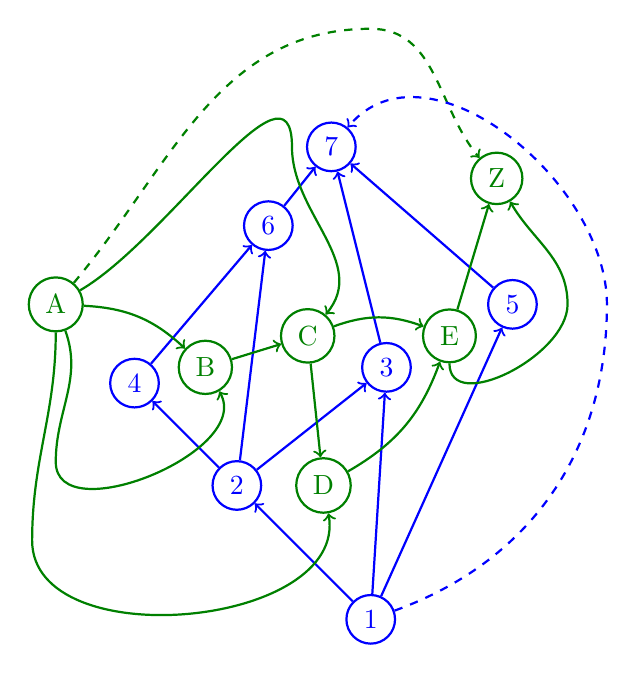
\begin{tikzpicture}[be/.style = {thick, Blue, ->}, ge/.style = {thick, Green, ->},
			bn/.style = {Blue, thick, circle, draw}, gn/.style = {Green, thick, circle, draw}]
			\node[bn] (1) at (0,0) {1};
			\node[bn] (2) at (-1.7, 1.7) {2};
			\node[bn] (3) at (.2, 3.2) {3};
			\node[bn] (4) at (-3, 3) {4};
			\node[bn] (5) at (1.8, 4) {5};
			\node[bn] (6) at (-1.3, 5) {6};
			\node[bn] (7) at (-.5, 6) {7};
			\node[gn] (A) at (-4, 4) {A};
			\node[gn] (B) at (-2.1, 3.2) {B};
			\node[gn] (C) at (-.8, 3.6) {C};
			\node[gn] (D) at (-.6, 1.7) {D};
			\node[gn] (E) at (1, 3.6) {E};
			\node[gn] (Z) at (1.6, 5.6) {Z};
			\draw[be] (1) -- (2);
			\draw[be] (1) -- (3);
			\draw[be] (1) -- (5);
			\draw[be] (2) -- (4);
			\draw[be] (2) -- (6);
			\draw[be] (2) -- (3);
			\draw[be] (5) -- (7);
			\draw[be] (3) -- (7);
			\draw[be] (6) -- (7);
			\draw[be] (4) -- (6);
			\draw[ge, bend left = 20] (A) edge (B);
			\draw[ge] (B) -- (C);
			\draw[ge] (C) -- (D);
			\draw[ge] (E) -- (Z);
			\draw[ge, bend right = 20] (D) edge (E);
			\draw[ge, bend left = 20] (C) edge (E);
			\draw[ge] (A) to[out=290, in=90] (-4, 2) to[out=270, in=300] (B);
			\draw[ge] (A) to[out=270, in=90] (-4.3, 1) to[out=270, in=280] (D);
			\draw[ge] (A) to[out=30, in=90] (-1, 6) to[out=270, in=50] (C);
			\draw[ge] (E) to[out=270, in=270] (2.5, 4) to[out=90, in=300] (Z);
			\draw[ge, dashed] (A) to[out=50, in=180] (0, 7.5) to[out=0, in=130] (Z);
			\draw[be, dashed] (1) to[out=20, in=270] (3, 4) to[out=90, in=50] (7);
		\end{tikzpicture}
	\end{subfigure}
	\begin{subfigure}{0.45\textwidth}\centering
		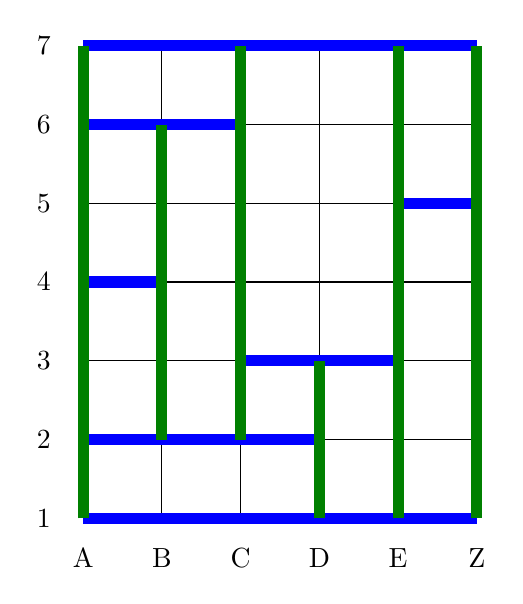
\begin{tikzpicture}[b/.style = {line width = 4, Blue}, g/.style = {line width = 4, Green}]
			\draw (1,1) -- (1,7);
			\draw (2,1) -- (2,7);
			\draw (3,1) -- (3,7);
			\draw (4,1) -- (4,7);
			\draw (5,1) -- (5,7);
			\draw (6,1) -- (6,7);
			\draw (1,1) -- (6,1);
			\draw (1,2) -- (6,2);
			\draw (1,3) -- (6,3);
			\draw (1,4) -- (6,4);
			\draw (1,5) -- (6,5);
			\draw (1,6) -- (6,6);
			\draw (1,7) -- (6,7);
			\draw[b] (1,1) -- (6,1);
			\draw[b] (1,2) -- (4,2);
			\draw[b] (3,3) -- (5,3);
			\draw[b] (1,4) -- (2,4);
			\draw[b] (5,5) -- (6,5);
			\draw[b] (1,6) -- (3,6);
			\draw[b] (1,7) -- (6,7);
			\draw[g] (1,1) -- (1,7);
			\draw[g] (2,2) -- (2,6);
			\draw[g] (3,2) -- (3,7);
			\draw[g] (4,1) -- (4,3);
			\draw[g] (5,1) -- (5,7);
			\draw[g] (6,1) -- (6,7);
			\node at (.5, 1) {1};
			\node at (.5, 2) {2};
			\node at (.5, 3) {3};
			\node at (.5, 4) {4};
			\node at (.5, 5) {5};
			\node at (.5, 6) {6};
			\node at (.5, 7) {7};
			\node at (1,.5) {A};
			\node at (2,.5) {B};
			\node at (3,.5) {C};
			\node at (4,.5) {D};
			\node at (5,.5) {E};
			\node at (6,.5) {Z};
		\end{tikzpicture}
	\end{subfigure}
	\caption{An overview of the construction by Algorithm RectangleVisibilityRep.}
\end{figure}

\section{Grid Contact graphs}

\begin{defn}
	A graph is a \textbf{Grid Intersection graph} if it has an intersection \\ representation by vertical and horizontal segments in which no two segments of the same direction share a point (in other words, all vertical, as well as all horizontal, segments are pairwise disjoint). A graph is a \textbf{Grid Contact} graph if it has a Grid Intersection representation in which no two segments cross, i.e., any two non-disjoint segments only touch each other.
\end{defn}

\begin{prop}
	Every grid intersection graph is bipartite. Moreover, every grid contact graph is planar.
\end{prop}

\begin{proof}
	The first claim is a simple observation. For the second claim, note that grid contact graphs form a subclass of triangle-free contact graphs of arc-connected regions in the plane. All such graphs are planar, since a non-crossing drawing can be constructed from a contact representation by selecting a point inside each region to represent its vertex, and connecting it to the contact points with the adjacent regions by curves inside the region.
\end{proof}

\begin{thm}
	Every planar bipartite graph is a grid contact graph.
	\label{thm-3}
\end{thm}

\begin{proof}
	Given a planar bipartite graph $G = (A \cup B, E)$, consider a non-crossing drawing and extend it to a non-crossing drawing of a supergraph $G' = (A' \cup B' , E')$ such that
	
	\begin{itemize}
		\item $G$ is an induced subgraph of $G'$,
		\item every face of the drawing of $G'$ is bounded by a cycle of length 4 (i.e., $G'$ is a so called quadrangulation),
		\item every vertex of $G'$ has degree greater than $2$, and
		\item no vertex of $B$ is on the boundary of the outerface of $G'$. 
	\end{itemize}
	
	Then construct the graph $\bar{G} = (A', \bar{E})$ by putting $\bar{E}$ the diagonals of the faces of $G'$ connecting their $A'$-vertices. It can be easily seen that $G$ is vertex 2-connected and that the faces of $\bar{G}$ are in 1-1 correspondence with the vertices of $B'$. Thus the segments of a rectangle visibility representation of $\bar{G}$ constructed as in the proof of Theorem \ref{thm-2} form a grid contact representation of $G'$ . Note the technical detail that the vertex (of $B'$) that corresponds to the outerface of $\bar{G}$ is represented by two vertical segments, not one. But this vertex does not belong to $B$, and so the segments corresponding to the vertices of $G$ form a grid contact representation of $G$.
\end{proof}

\begin{figure}[!ht]
	\begin{subfigure}{0.45\textwidth}\centering
		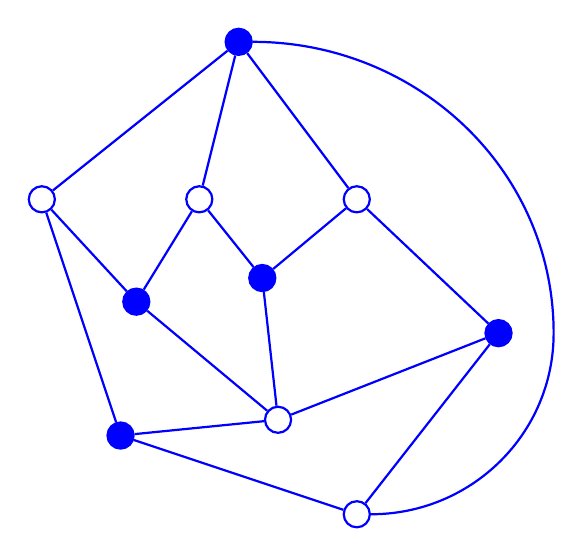
\begin{tikzpicture}[main/.style = {draw, circle, thick, Blue},
			edge/.style = {thick, Blue},
			fil/.style = {thick, fill, draw, circle, Blue}]
			\node[main] (1) at (0,0) {};
			\node[fil] (2) at (1.8, 2.3) {};
			\node[fil] (3) at (-3, 1) {};
			\node[main] (4) at (-1, 1.2) {};
			\node[fil] (5) at (-1.2, 3) {};
			\node[fil] (6) at (-2.8, 2.7) {};
			\node[main] (7) at (-4, 4) {};
			\node[main] (8) at (-2, 4) {};
			\node[main] (9) at (0, 4) {};
			\node[fil] (10) at (-1.5, 6) {};
			\draw[edge] (1) -- (2);
			\draw[edge] (1) -- (3);
			\draw[edge] (3) -- (4);
			\draw[edge] (2) -- (4);
			\draw[edge] (4) -- (5);
			\draw[edge] (4) -- (6);
			\draw[edge] (2) -- (9);
			\draw[edge] (9) -- (10);
			\draw[edge] (8) -- (10);
			\draw[edge] (7) -- (10);
			\draw[edge] (3) -- (7);
			\draw[edge] (6) -- (7);
			\draw[edge] (5) -- (8);
			\draw[edge] (6) -- (8);
			\draw[edge] (5) -- (9);
			\draw[edge] (1) to[out=0, in=270] (2.5, 2.3) to[out=90, in=0] (10);
		\end{tikzpicture}
		\caption{The graph $G'$.}
	\end{subfigure}
	\begin{subfigure}{0.53\textwidth}\centering
		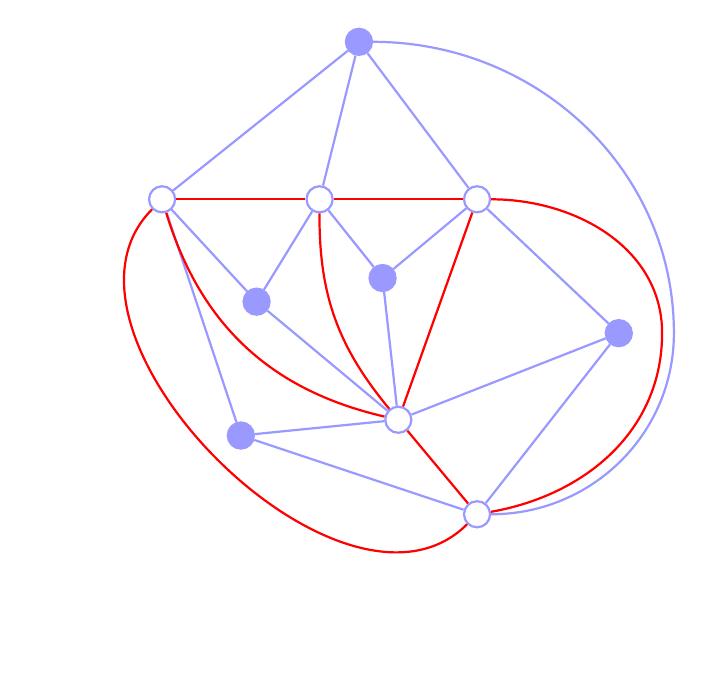
\begin{tikzpicture}[main/.style = {draw, circle, thick, Blue!40},
			edge/.style = {thick, Blue!40},
			fil/.style = {thick, fill, draw, circle, Blue!40},
			red/.style = {thick, Red}]
			\node[main] (1) at (0,0) {};
			\node[fil] (2) at (1.8, 2.3) {};
			\node[fil] (3) at (-3, 1) {};
			\node[main] (4) at (-1, 1.2) {};
			\node[fil] (5) at (-1.2, 3) {};
			\node[fil] (6) at (-2.8, 2.7) {};
			\node[main] (7) at (-4, 4) {};
			\node[main] (8) at (-2, 4) {};
			\node[main] (9) at (0, 4) {};
			\node[fil] (10) at (-1.5, 6) {};
			\draw[edge] (1) -- (2);
			\draw[edge] (1) -- (3);
			\draw[edge] (3) -- (4);
			\draw[edge] (2) -- (4);
			\draw[edge] (4) -- (5);
			\draw[edge] (4) -- (6);
			\draw[edge] (2) -- (9);
			\draw[edge] (9) -- (10);
			\draw[edge] (8) -- (10);
			\draw[edge] (7) -- (10);
			\draw[edge] (3) -- (7);
			\draw[edge] (6) -- (7);
			\draw[edge] (5) -- (8);
			\draw[edge] (6) -- (8);
			\draw[edge] (5) -- (9);
			\draw[edge] (1) to[out=0, in=270] (2.5, 2.3) to[out=90, in=0] (10);
			\draw[red] (1) edge (4);
			\draw[red, bend right = 30] (7) edge (4);
			\draw[red, bend left = 90] (1) edge (7);
			\draw[red, bend right = 20] (8) edge (4);
			\draw[red] (4) edge (9);
			\draw[red] (8) edge (9);
			\draw[red] (1) to[out=10, in=270] (2.35, 2.3) to[out=90, in=0] (9);
			\draw[red] (7) edge (8);
		\end{tikzpicture}
		\caption{The graph $G$.}
	\end{subfigure}
	\caption{An illustration to the proof of Theorem \ref{thm-3}.}
\end{figure}
	
	\chapter{Schnyder woods}

\section{Canonical ordering}

\begin{defn}
	Given a plane triangulation (i.e., a non-crossing embedding of a trian-\\gulation in the plane, which means that the outerface is fixed) $G = (V, E)$, a canonical ordering of it is a numbering $1, 2, \dots, n$ of its vertices such that
	
	\begin{enumerate}[i)]
		\item the vertices of the outerface are $1, 2$ and $n = |V|$,
		\item for every $i = 3, 4, \dots, n - 1$,
		\begin{enumerate}[a)]
			\item the graph $G_i = G[1, 2, \dots, i]$ is vertex 2-connected,
			\item all vertices $j \leq i$ are drawn inside (or on the boundary) of the embedding of $G_i$ inherited from the embedding of $G$,
			\item all vertices $j > i$ are drawn outside the embedding of $G_i$ inherited from the embedding of $G$,
			\item the neighbors of vertex $i + 1$ in $G_i$ are lying consecutively on the boundary of $G_i$.
		\end{enumerate}
	\end{enumerate}
\end{defn}

\begin{thm}
	Every triangulation has a canonical ordering.
\end{thm}

\begin{proof}
	By induction from $n$ downto $3$, assign the numbers to the vertices. Once $n, n - 1, \dots, i + 1$ are assigned, choose as vertex $i$ such a vertex on the boundary of $G_i$ whose deletion from $G_i$ leaves $G_{i-1}$ vertex 2-connected. The only obstacle to preserving 2-connectedness is if $i$ would be incident to a diagonal edge (an edge with both end-vertices on the boundary of the outerface, but which itself is not a part of the boundary). But there is always a vertex which is not incident with any diagonal (to observe this, consider a vertex which is incident with a shortest possible diagonal, with the length of a diagonal being measured by the number of vertices of the boundary that it cuts off of $G_i$). So assign $i$ to a vertex (there may be more options) which is not incident to any diagonal. Then a), b) and c) are fulfilled for $G_{i-1}$. Note that d) follows from b) and c).
\end{proof}

\section{Schnyder woods}

\begin{algorithm}[!ht]
	\caption{Schnyder}
	\begin{algorithmic}[1]
		\Require A plane triangulation $G = (V, E)$ and a canonical ordering of it.
		\For{$i := 3 \dots n -1$}
			\State set $b(i)$ to be the leftmost neighbor of $i$ on the boundary of $G_{i-1}$, direct the edge $ib(i)$ in this direction and color it blue;
			\State set $g(i)$ to be the rightmost neighbor of $i$ on the boundary of $G_{i-1}$, direct the edge $ig(i)$ in this direction and color it green;
			\State set $r(i)$ to be the neighbor of $i$ with the highest number, direct the edge $ig(i)$ in this direction and color it red
		\EndFor
		\State \Return the orientation of $G$, the coloring of its edges and the mappings $b, g$ and $r$.
	\end{algorithmic}
\end{algorithm}

\begin{figure}[!ht]\centering
	\begin{subfigure}{0.45\textwidth}\centering
		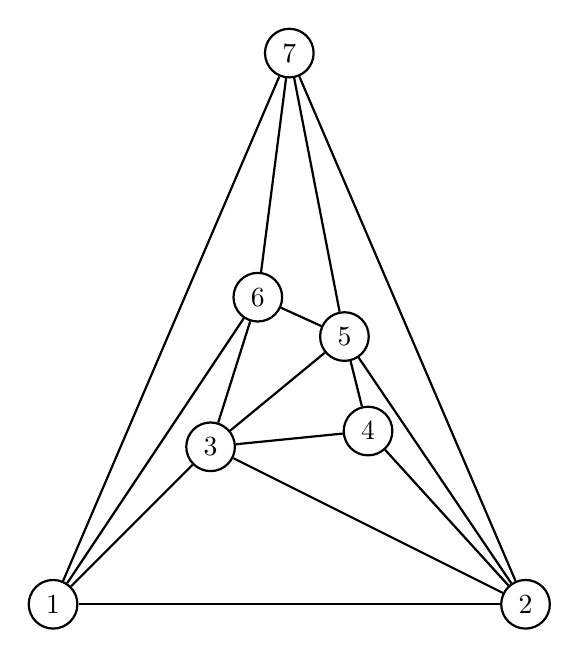
\begin{tikzpicture}[main/.style = {draw, circle, thick}]
			\node[main] (1) at (-1,-1) {1};
			\node[main] (2) at (5,-1) {2};
			\node[main] (3) at (1,1) {3};
			\node[main] (4) at (3, 1.2) {4};
			\node[main] (5) at (2.7, 2.4) {5};
			\node[main] (6) at (1.6, 2.9) {6};
			\node[main] (7) at (2, 6) {7};
			\draw[thick] (1) edge (3);
			\draw[thick] (1) edge (2);
			\draw[thick] (1) edge (7);
			\draw[thick] (1) edge (6);
			\draw[thick] (6) edge (3);
			\draw[thick] (4) edge (3);
			\draw[thick] (5) edge (3);
			\draw[thick] (2) edge (3);
			\draw[thick] (2) edge (4);
			\draw[thick] (2) edge (5);
			\draw[thick] (2) edge (7);
			\draw[thick] (5) edge (4);
			\draw[thick] (5) edge (6);
			\draw[thick] (7) edge (6);
			\draw[thick] (7) edge (5);
		\end{tikzpicture}
	\end{subfigure}
	\begin{subfigure}{0.45\textwidth}\centering
		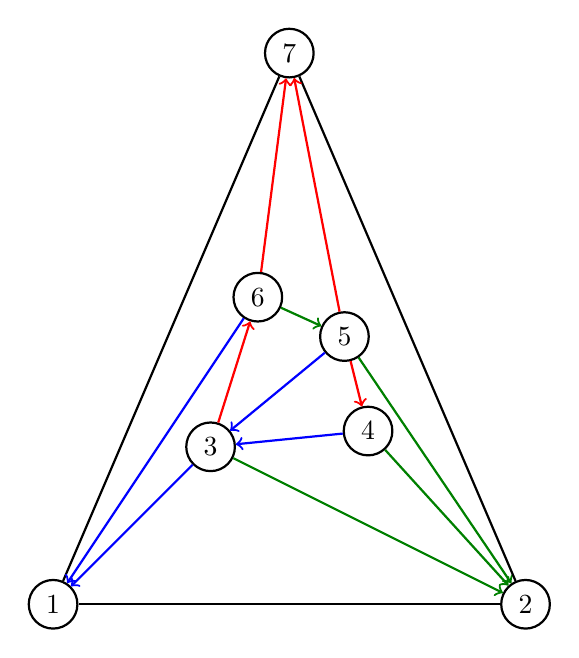
\begin{tikzpicture}[main/.style = {draw, circle, thick}]
			\node[main] (1) at (-1,-1) {1};
			\node[main] (2) at (5,-1) {2};
			\node[main] (3) at (1,1) {3};
			\node[main] (4) at (3, 1.2) {4};
			\node[main] (5) at (2.7, 2.4) {5};
			\node[main] (6) at (1.6, 2.9) {6};
			\node[main] (7) at (2, 6) {7};
			\draw[thick, ->, color=Blue] (3) edge (1);
			\draw[thick] (1) edge (2);
			\draw[thick] (1) edge (7);
			\draw[thick, ->, color=Blue] (6) edge (1);
			\draw[thick, ->, color=Red] (3) edge (6);
			\draw[thick, ->, color=Blue] (4) edge (3);
			\draw[thick, ->, color=Blue] (5) edge (3);
			\draw[thick, ->, color=Green] (3) edge (2);
			\draw[thick, ->, color=Green] (4) edge (2);
			\draw[thick, ->, color=Green] (5) edge (2);
			\draw[thick] (2) edge (7);
			\draw[thick, ->, color=Red] (5) edge (4);
			\draw[thick, ->, color=Green] (6) edge (5);
			\draw[thick, ->, color=Red] (6) edge (7);
			\draw[thick, ->, color=Red] (5) edge (7);
		\end{tikzpicture}
	\end{subfigure}
	\caption{An illustration to canonical orderings and Schnyder woods.}
\end{figure}

\begin{thm}
	The blue edges form a tree rooted in vertex 1 and spanning the vertices $1, 3, \dots, n - 1$, the green edges form a tree rooted in vertex 2 and spanning the vertices $2, 3, \dots, n - 1$, and the red edges form a tree rooted in vertex n and spanning the vertices $3, \dots , n$. Every edge of $G$, except of $12, 1n, 2n$, belongs to exactly one of these trees.
\end{thm}

\begin{proof}
	Clear from the construction and properties of canonical orderings.
\end{proof}

\begin{cor}
	The edges of a planar triangulation can be partitioned into edge sets of 3 trees and a triangle. Such a collection of three trees is called a \textbf{Schnyder wood} of $G$.
\end{cor}

\begin{figure}[!ht]\centering
	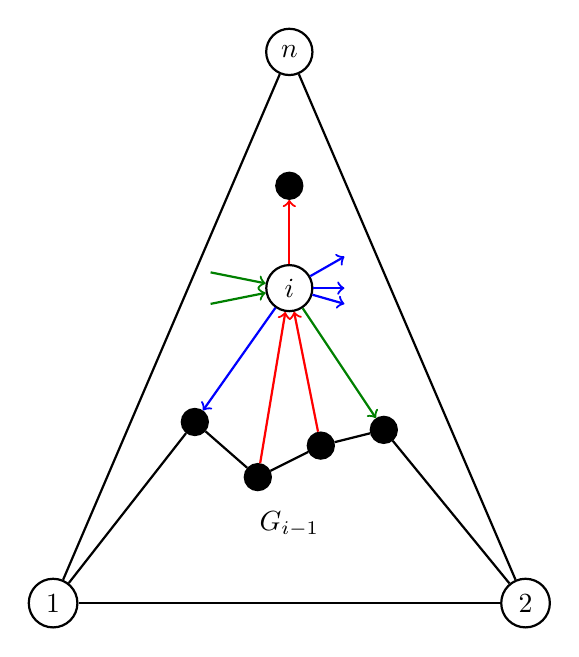
\begin{tikzpicture}[main/.style = {draw, circle, thick}]
		\node[main] (1) at (-1,-1) {1};
		\node[main] (2) at (5,-1) {2};
		\node[main, fill] (3) at (.8,1.3) {};
		\node[main, fill] (4) at (3.2, 1.2) {};
		\node[main, fill] (5) at (2.4, 1) {};
		\node[main, fill] (6) at (1.6, 0.6) {};
		\node[main] (n) at (2, 6) {$n$};
		\node[main] (i) at (2, 3) {$i$};
		\node[main, fill] (7) at (2, 4.3) {};
		\node (G) at (2, 0) {$G_{i-1}$};
		\draw[thick] (1) edge (3);
		\draw[thick] (1) edge (2);
		\draw[thick] (1) edge (n);
		\draw[thick] (6) edge (3);
		\draw[thick] (2) edge (4);
		\draw[thick] (2) edge (n);
		\draw[thick] (5) edge (4);
		\draw[thick] (5) edge (6);		
		\draw[thick, color=Blue, ->] (i) edge (3);
		\draw[thick, color=Red, ->] (6) edge (i);
		\draw[thick, color=Red, ->] (5) edge (i);
		\draw[thick, color=Green, ->] (i) edge (4);
		\draw[thick, color=Red, ->] (i) edge (7);
		\draw[thick, color=Green, ->] (1, 3.2) -- (i);
		\draw[thick, color=Green, ->] (1, 2.8) -- (i);
		\draw[thick, color=Blue, ->] (i) -- (2.7, 3.4);
		\draw[thick, color=Blue, ->] (i) -- (2.7, 2.8);
		\draw[thick, color=Blue, ->] (i) -- (2.7, 3);
	\end{tikzpicture}
	\caption{The rotation scheme of incoming and outgoing edges around a vertex in the Schnyder wood.}
\end{figure}

\begin{prop}
	Locally around every inner vertex of $G$, we see (in the counter-clock-wise order) one outgoing blue edge, several (or none) incoming red edges, one outgoing green edge, several (or none) incoming blue edges, one outgoing red edge, and several (or none) incoming green edges.
\end{prop}

\section{Triangle contact representations}

\begin{thm}[de Fraysseix, Ossona de Mendez, Rosenstiehl]
	Every planar graph is a contact graph of isosceles triangles with horizontal bases.
\end{thm}

\begin{proof}
	It suffices to prove the theorem for triangulations, since every planar graph is an induced subgraph of a triangulation. Given a triangulation $G = (V, E)$, fix an embedding and consider a canonical ordering with respect to this embedding, and run algorithm Schnyder on this canonical ordering. Draw $n + 1 = |V| + 1$ parallel horizontal lines and build triangles as follows:
	
	\begin{enumerate}
		\item Triangle $T_i$ is isosceles and its base lies on the $i$-th line,
		\item The peaks of $T_1$ and $T_2$ are on the $(n + 1)$-st line, the left corner of $T_2$ touches the right side of $T_1$,
		\item For every $i = 1, 2, \dots, n$, the left corner of $T_i$ lies on the right side of $T_{b(i)}$, the right corner of $T_i$ lies on the left side of $T_{g(i)}$ and the peak of $T_i$ lies on the $r(i)$-th line (on the $(n + 1)$-st line for $i = n$).
	\end{enumerate}
	
	Construct the triangles from $T_1$ to $T_n$. For $T_1$, only the lines supporting its base and peak are prescribed, the triangle is free otherwise. For $T_2$, the freedom is restricted only to the position of the right corner (which then determines the position of the peak). For $i > 2$, the triangles are then determined uniquely. The loop invariant of this inductive construction is that for $i > 1$, the upper boundary of the union of triangles $T_1 , T_2 , \dots, T_i$ is connected and the order in which the triangles appear on this boundary is the same as the order of the corresponding vertices appearing on the upper boundary of $G_i$. This implies that $T_i$ is always placed in the way that it is touching the respective neighbors, but not crossing any triangle of the representation.
\end{proof}

\begin{figure}
	\begin{subfigure}{0.45\textwidth}\centering
		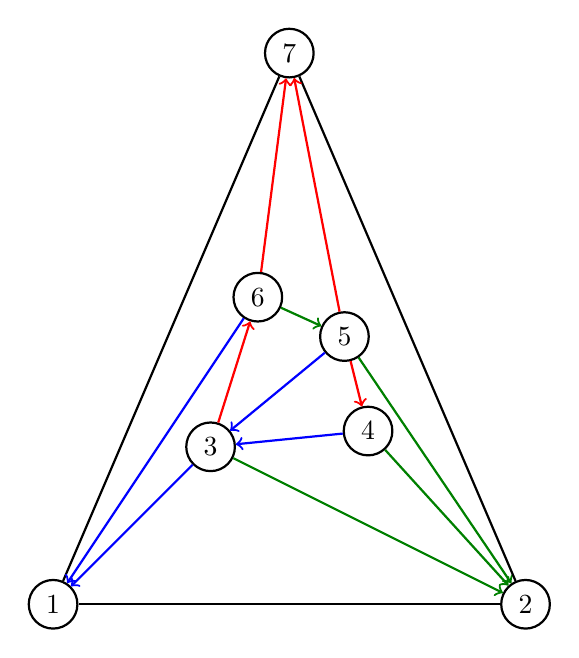
\begin{tikzpicture}[main/.style = {draw, circle, thick}]
			\node[main] (1) at (-1,-1) {1};
			\node[main] (2) at (5,-1) {2};
			\node[main] (3) at (1,1) {3};
			\node[main] (4) at (3, 1.2) {4};
			\node[main] (5) at (2.7, 2.4) {5};
			\node[main] (6) at (1.6, 2.9) {6};
			\node[main] (7) at (2, 6) {7};
			\draw[thick, ->, color=Blue] (3) edge (1);
			\draw[thick] (1) edge (2);
			\draw[thick] (1) edge (7);
			\draw[thick, ->, color=Blue] (6) edge (1);
			\draw[thick, ->, color=Red] (3) edge (6);
			\draw[thick, ->, color=Blue] (4) edge (3);
			\draw[thick, ->, color=Blue] (5) edge (3);
			\draw[thick, ->, color=Green] (3) edge (2);
			\draw[thick, ->, color=Green] (4) edge (2);
			\draw[thick, ->, color=Green] (5) edge (2);
			\draw[thick] (2) edge (7);
			\draw[thick, ->, color=Red] (5) edge (4);
			\draw[thick, ->, color=Green] (6) edge (5);
			\draw[thick, ->, color=Red] (6) edge (7);
			\draw[thick, ->, color=Red] (5) edge (7);
		\end{tikzpicture}
	\end{subfigure}
	\begin{subfigure}{0.45\textwidth}\centering
		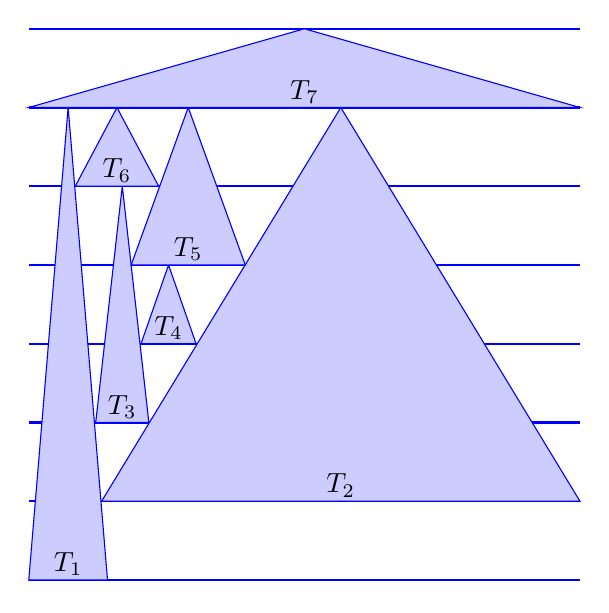
\begin{tikzpicture}
			\draw[Blue, thick] (0,0) -- (7,0);
			\draw[Blue, thick] (0,1) -- (7,1);
			\draw[Blue, thick] (0,2) -- (7,2);
			\draw[Blue, thick] (0,3) -- (7,3);
			\draw[Blue, thick] (0,4) -- (7,4);
			\draw[Blue, thick] (0,5) -- (7,5);
			\draw[Blue, thick] (0,6) -- (7,6);
			\draw[Blue, thick] (0,7) -- (7,7);
			\draw[Blue, fill=Blue!20] (0,0) -- (1,0) -- (0.5,6) -- cycle;
			\draw[Blue, fill=Blue!20] (0.925,1) -- (7,1) -- (3.9625,6) -- cycle;
			\draw[Blue, fill=Blue!20] (0.85,2) -- (1.525,2) -- (1.1875,5) -- cycle;
			\draw[Blue, fill=Blue!20] (1.425,3) -- (2.125,3) -- (1.775,4) -- cycle;
			\draw[Blue, fill=Blue!20] (1.3,4) -- (2.75,4) -- (2.025,6) -- cycle;
			\draw[Blue, fill=Blue!20] (0.59,5) -- (1.65,5) -- (1.12,6) -- cycle;
			\draw[Blue, fill=Blue!20] (0,6) -- (7,6) -- (3.5,7) -- cycle;
			\node at (.5, .2) {$T_1$};
			\node at (3.9625, 1.2) {$T_2$};
			\node at (1.1875, 2.2) {$T_3$};
			\node at (1.775, 3.2) {$T_4$};
			\node at (2.025, 4.2) {$T_5$};
			\node at (1.12, 5.2) {$T_6$};
			\node at (3.5, 6.2) {$T_7$};
		\end{tikzpicture}
	\end{subfigure}
	\caption{An illustration to contact representations by isosceles triangles.}
\end{figure}

\section{Drawing planar graphs on small grids}

\begin{thm}
	Every planar $n$-vertex graph allows a straight-line non-crossing embedding on a grid of size $n \times n$.
\end{thm}

\begin{proof}
	It suffices to prove the theorem for planar triangulations. Given a triangulation $G = (V, E)$, fix an embedding and consider a canonical ordering with respect to this embedding, and run algorithm Schnyder on this canonical ordering. Assign barycentric coordinates $(x_i , y_i , z_i)$ to every vertex $i = 3, 4, \dots, n - 1$ as follows (see Fig. \ref{coord} for illustration): The triangle $12n$ is divided into three regions by the blue, green and red directed paths from $i$ to the roots of the trees in the Schnyder wood. Let $x_i$ be the number of vertices in the region bounded by the blue and green paths and the side $12$, with the vertices on the green path being counted in, but not the vertices of the blue path. Similarly, $y_i$ is the number of vertices in the region bounded by the blue and red paths and the side $1n$, with the vertices on the blue path being counted in, but not the vertices of the red path, and $z_i$ is the number of vertices in the region bounded by the red and green paths and the side $n2$, with the vertices on the red path being counted in, but not the vertices of the green one. Vertex $i$ itself is not counted in neither of the regions.

	\begin{figure}[!ht]\centering
		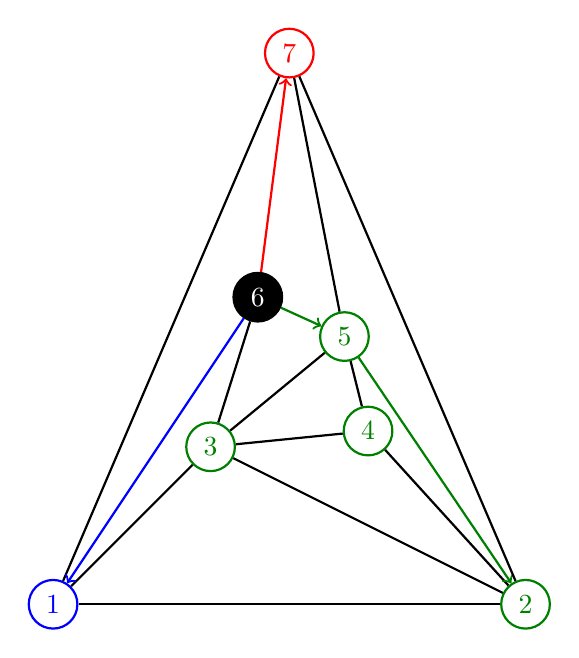
\begin{tikzpicture}[main/.style = {draw, circle, thick}]
			\node[main, Blue] (1) at (-1,-1) {1};
			\node[main, Green] (2) at (5,-1) {2};
			\node[main, Green] (3) at (1,1) {3};
			\node[main, Green] (4) at (3, 1.2) {4};
			\node[main, Green] (5) at (2.7, 2.4) {5};
			\node[main, fill, Black] (6) at (1.6, 2.9) {\textcolor{white}{6}};
			\node[main, Red] (7) at (2, 6) {7};
			\draw[thick] (1) edge (3);
			\draw[thick] (1) edge (2);
			\draw[thick] (1) edge (7);
			\draw[thick, color=Blue, ->] (6) edge (1);
			\draw[thick] (6) edge (3);
			\draw[thick] (4) edge (3);
			\draw[thick] (5) edge (3);
			\draw[thick] (2) edge (3);
			\draw[thick] (2) edge (4);
			\draw[thick, color=Green, ->] (5) edge (2);
			\draw[thick] (2) edge (7);
			\draw[thick] (5) edge (4);
			\draw[thick, color=Green, ->] (6) edge (5);
			\draw[thick, color=Red, ->] (6) edge (7);
			\draw[thick] (7) edge (5);
		\end{tikzpicture}
		\caption{An illustration to the definition of barycentric coordinates from Schnyder woods. The green vertices are counted for the definition of $x_6$, the blue one for the definition of $y_6$ and the red one for the definition of $z_6$. Vertex 6 itself does not contribute to any of the coordinates.}
		\label{coord}
	\end{figure}

	Then every vertex except of $i$ belongs to exactly one of the regions, end hence
	
	$$
	x_i + y_i + z_i = n - 1
	$$
	
	for every $i$. For $i = 1, 2$, and $n$, we set
	
	$$
	\begin{array}{lll}
		x_1 = 0,   &y_1 = 0,   &z_1 = n - 1\\
		x_2 = 0,   &y_2 = n-1, &z_2 = 0\\
		x_n = n-1, &y_n = 0,   & z_n = 0 	
	\end{array}
	$$
	
	Place vertex $i$ in the point with barycentric coordinates $(x_i , y_i , z_i)$ in a triangular $n \times n \times n$ grid (the lines of the grid have coordinates $0, 1, \dots, n - 1$). Draw the edges of $G$ as straight-line segments
	connecting their vertices.
	
	\begin{claim}
		Consider a vertex $i \in \{3, 4, \dots, n - 1\}$. In the drawing constructed as above, the blue edge $ib(i)$ is directed into the bottom-left sextant of $i$, the edge $ig(i)$ is directed into the bottom-right sextant of $i$, and the edge $ir(i)$ is directed into the top sextant of $i$.
		\label{claim-1}
	\end{claim}
	
	\begin{proof}[Proof of claim]
		From the definition of the coordinates, it follows that $xb(i) \leq x_i$, $yb(i) < y_i$ and $zb(i) \geq z_i$, and this implies the direction of the edge $ib(i)$. Similarly for the others.
	\end{proof}
	
	\begin{claim}
		The rotation scheme of the edges around each vertex $i$ in the barycentric drawing is the same as the rotation scheme of the edges incident to the same vertex in $G$.
	\end{claim}
	
	\begin{proof}[Proof of claim]
		This follows by application of Claim \ref{claim-1} to the other end-vertices of the edges directed into $i$.
	\end{proof}
	
	\begin{claim}
		The barycentric drawing is non-crossing and topologically equivalent to the plane embedding of $G$ we started with.
	\end{claim}
	
	\begin{proof}[Proof of claim]
		If the rotation schemes for all vertices of drawings of two 3-connected graphs are the same and one of the drawings is non-crossing, then so is the other one, and the drawings are topologically equivalent.
	\end{proof}
\end{proof}

\section{Boxicity of graphs}

\begin{defn}
	The \textbf{boxicity} of a graph $G$, denoted by $\text{box}(G)$, is the smallest integer $d$ such that $G$ is an intersection graph of boxes in $\R^d$ (i.e., of $d$-dimensional intervals in the $d$-dimensional Euclidean space).
\end{defn}

\begin{prop}
For every graph $G = (V, E)$, its boxicity is a correctly defined finite number. It equals the minimum number of interval graphs whose intersection is equal to $G$, i.e., the minimum number $d$ for which sets $E_i \subseteq \binom{V}{2} , i = 1, 2, \dots, d$ exist, such that $E = \cup_{i=1}^d E_i$ and $(V, E_i)$ is an interval graph for every $i = 1, 2, \dots, d$.
\end{prop}

\begin{proof}
	An exercise. Proof the claim for graphs $G$ which are not complete. For a complete graph, the boxicity is $0$, which corresponds to the fact that the intersection of an empty set of subsets of a ground set ($E$, in this case) is by default set to be equal to the ground set itself.
\end{proof}

\section{Grid intersection graphs}

\begin{defn}
	A graph is a \textbf{Grid Intersection graph} if it has an intersection repre-\\sentation by vertical and horizontal segments in which no two segments of the same direction share a point (in other words, all vertical, as well as all horizontal, segments are pairwise disjoint).
\end{defn}

It is easy to observe that every grid intersection graph has a grid intersection repre-\\sentation in which no two segments lie on the same line. Moreover, the exact $x$-coordinates of the vertical segments, nor the exact $y$-coordinates of the horizontal ones, are important, only their linear orders. Thus we assume that our bipartite graph $G = (A \cup B, E)$ has its vertices linearly ordered within the classes of bipartition, $A = \{a_1 , a_2 , \dots, a_n\}, B = \{b_1 , b_2 \dots, b_m\}$. We further assume that the vertices of $A$ are to be represented by vertical segments and the vertices of $B$ by horizontal ones. We say that a grid intersection representation respects the orders of $A$ and $B$ if for every $i < j$, the $x$-coordinate of $a_i$ is smaller than the $x$-coordinate of $a_j$, and the $y$-coordinate of $b_i$ is smaller than the $y$-coordinate of $b_j$.

\begin{thm}
	The graph $G = (A \cup B, E)$ has a grid intersection representation that respects the linear orders of $A$ and $B$ if and only if there are no 6 indices $i < j < k, \alpha < \beta < \gamma$ such that $a_i b_\beta , a_k b_\beta , a_j b_\alpha , a_j b_\gamma$ are edges of $G$ and $a_j b_\beta$ is not. Such a configuration of 6 vertices is called a \textbf{volswagen} in $G$.
	\label{thm-5}
\end{thm}

\begin{proof}
	Exercise.
\end{proof}

It is easy (i.e., decidable in polynomial time) to check if a bipartite graph contains a volkswagen with respect to given linear orderings of the vertices in its classes of bipartition. We will see in the last class that it is NP-complete to decide if a given bipartite graph is a grid intersection graph, which means that it is NP-complete to decide if a given bipartite graph allows linear orderings of its classes of bipartition with respect to which there is no volkswagen. The following problem is thus quite interesting in this context.

\textbf{Open problem:} Given a bipartite graph with one class of bipartition linearly ordered. How difficult is to decide if the other class of bipartition can be linearly ordered so that there is no volkswagen with respect to these orderings?

\begin{thm}[Bellantoni, Hartman, Przytycka, Whitesides]
	Every bipartite graph of boxicity $2$ is a grid intersection graph.
\end{thm}

\begin{figure}[!ht]\centering
	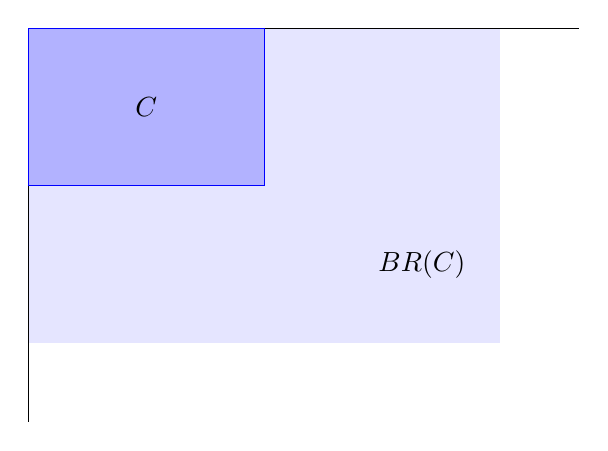
\begin{tikzpicture}
		\draw[black!0, fill=blue!10] (0,-2) rectangle (6,2);
		\draw (0,2) -- (7,2);
		\draw (0,2) -- (0, -3);
		\draw[blue, fill=blue!30] (0,0) rectangle (3,2);
		\node at (1.5, 1) {$C$};
		\node at (5,-1) {$BR(C)$};
	\end{tikzpicture}
	\caption{An illustration to the definition of region $BR(C)$.}
\end{figure}

\begin{proof}[Sketch of proof]
	Suppose $G = (A \cup B, E)$ is a bipartite graph and let $\mathcal{R} = \{R(u) : u \in A \cup B\}$ be an intersection representation of $G$ by axes-parallel rectangles in the plane. For a rectangle $C$ in the plane, we define regions $BL(C)$, $BR(C)$, $TL(C)$, $TR(C)$ as follows: $BR(C)$ contains all points with $x$-coordinate greater than the $x$-coordinate of the left side of $C$, with $y$-coordinate smaller than the $y$-coordinate of the top side of $C$, but which do not lie inside the rectangle $C$. The other regions ($BL$ standing for Bottom-Left, $TL$ standing for Top-Left, and $TR$ standing for Top-Right) are defined in a similar way. Then define two binary relations, one on $A$, the other one on $B$, as follows
	
	\begin{claim}
		Both relations $<_R$ and $<_L$ are antireflexive, antisymmetric and acyclic. It follows that the transitive closures $<_{R}^T$ and $<_{L}^T$ of $<_R$ and $<_L$, respectively, are partial orders.
	\end{claim}
	
	Let $<_R^\ast$ and $<_L^\ast$ be topological sortings of $<_R^T$ and $<_L^T$, respectively.
	
	\begin{claim}
		With respect to the linear orderings $<_R^\ast$ and $<_L^\ast$ of its classes of bipartition, $G$ has no volkswagens. Hence $G$ has a grid intersection representation respecting these orders by Theorem \ref{thm-5}.
	\end{claim}
\end{proof}
\end{document}

